% Options for packages loaded elsewhere
\PassOptionsToPackage{unicode}{hyperref}
\PassOptionsToPackage{hyphens}{url}
\PassOptionsToPackage{dvipsnames,svgnames,x11names}{xcolor}
%
\documentclass[
  letterpaper,
  DIV=11,
  numbers=noendperiod,
  oneside]{scrreprt}

\usepackage{amsmath,amssymb}
\usepackage{lmodern}
\usepackage{iftex}
\ifPDFTeX
  \usepackage[T1]{fontenc}
  \usepackage[utf8]{inputenc}
  \usepackage{textcomp} % provide euro and other symbols
\else % if luatex or xetex
  \usepackage{unicode-math}
  \defaultfontfeatures{Scale=MatchLowercase}
  \defaultfontfeatures[\rmfamily]{Ligatures=TeX,Scale=1}
\fi
% Use upquote if available, for straight quotes in verbatim environments
\IfFileExists{upquote.sty}{\usepackage{upquote}}{}
\IfFileExists{microtype.sty}{% use microtype if available
  \usepackage[]{microtype}
  \UseMicrotypeSet[protrusion]{basicmath} % disable protrusion for tt fonts
}{}
\makeatletter
\@ifundefined{KOMAClassName}{% if non-KOMA class
  \IfFileExists{parskip.sty}{%
    \usepackage{parskip}
  }{% else
    \setlength{\parindent}{0pt}
    \setlength{\parskip}{6pt plus 2pt minus 1pt}}
}{% if KOMA class
  \KOMAoptions{parskip=half}}
\makeatother
\usepackage{xcolor}
\usepackage[left=1in,marginparwidth=2.0666666666667in,textwidth=4.1333333333333in,marginparsep=0.3in]{geometry}
\setlength{\emergencystretch}{3em} % prevent overfull lines
\setcounter{secnumdepth}{5}
% Make \paragraph and \subparagraph free-standing
\ifx\paragraph\undefined\else
  \let\oldparagraph\paragraph
  \renewcommand{\paragraph}[1]{\oldparagraph{#1}\mbox{}}
\fi
\ifx\subparagraph\undefined\else
  \let\oldsubparagraph\subparagraph
  \renewcommand{\subparagraph}[1]{\oldsubparagraph{#1}\mbox{}}
\fi

\usepackage{color}
\usepackage{fancyvrb}
\newcommand{\VerbBar}{|}
\newcommand{\VERB}{\Verb[commandchars=\\\{\}]}
\DefineVerbatimEnvironment{Highlighting}{Verbatim}{commandchars=\\\{\}}
% Add ',fontsize=\small' for more characters per line
\usepackage{framed}
\definecolor{shadecolor}{RGB}{241,243,245}
\newenvironment{Shaded}{\begin{snugshade}}{\end{snugshade}}
\newcommand{\AlertTok}[1]{\textcolor[rgb]{0.68,0.00,0.00}{#1}}
\newcommand{\AnnotationTok}[1]{\textcolor[rgb]{0.37,0.37,0.37}{#1}}
\newcommand{\AttributeTok}[1]{\textcolor[rgb]{0.40,0.45,0.13}{#1}}
\newcommand{\BaseNTok}[1]{\textcolor[rgb]{0.68,0.00,0.00}{#1}}
\newcommand{\BuiltInTok}[1]{\textcolor[rgb]{0.00,0.23,0.31}{#1}}
\newcommand{\CharTok}[1]{\textcolor[rgb]{0.13,0.47,0.30}{#1}}
\newcommand{\CommentTok}[1]{\textcolor[rgb]{0.37,0.37,0.37}{#1}}
\newcommand{\CommentVarTok}[1]{\textcolor[rgb]{0.37,0.37,0.37}{\textit{#1}}}
\newcommand{\ConstantTok}[1]{\textcolor[rgb]{0.56,0.35,0.01}{#1}}
\newcommand{\ControlFlowTok}[1]{\textcolor[rgb]{0.00,0.23,0.31}{#1}}
\newcommand{\DataTypeTok}[1]{\textcolor[rgb]{0.68,0.00,0.00}{#1}}
\newcommand{\DecValTok}[1]{\textcolor[rgb]{0.68,0.00,0.00}{#1}}
\newcommand{\DocumentationTok}[1]{\textcolor[rgb]{0.37,0.37,0.37}{\textit{#1}}}
\newcommand{\ErrorTok}[1]{\textcolor[rgb]{0.68,0.00,0.00}{#1}}
\newcommand{\ExtensionTok}[1]{\textcolor[rgb]{0.00,0.23,0.31}{#1}}
\newcommand{\FloatTok}[1]{\textcolor[rgb]{0.68,0.00,0.00}{#1}}
\newcommand{\FunctionTok}[1]{\textcolor[rgb]{0.28,0.35,0.67}{#1}}
\newcommand{\ImportTok}[1]{\textcolor[rgb]{0.00,0.46,0.62}{#1}}
\newcommand{\InformationTok}[1]{\textcolor[rgb]{0.37,0.37,0.37}{#1}}
\newcommand{\KeywordTok}[1]{\textcolor[rgb]{0.00,0.23,0.31}{#1}}
\newcommand{\NormalTok}[1]{\textcolor[rgb]{0.00,0.23,0.31}{#1}}
\newcommand{\OperatorTok}[1]{\textcolor[rgb]{0.37,0.37,0.37}{#1}}
\newcommand{\OtherTok}[1]{\textcolor[rgb]{0.00,0.23,0.31}{#1}}
\newcommand{\PreprocessorTok}[1]{\textcolor[rgb]{0.68,0.00,0.00}{#1}}
\newcommand{\RegionMarkerTok}[1]{\textcolor[rgb]{0.00,0.23,0.31}{#1}}
\newcommand{\SpecialCharTok}[1]{\textcolor[rgb]{0.37,0.37,0.37}{#1}}
\newcommand{\SpecialStringTok}[1]{\textcolor[rgb]{0.13,0.47,0.30}{#1}}
\newcommand{\StringTok}[1]{\textcolor[rgb]{0.13,0.47,0.30}{#1}}
\newcommand{\VariableTok}[1]{\textcolor[rgb]{0.07,0.07,0.07}{#1}}
\newcommand{\VerbatimStringTok}[1]{\textcolor[rgb]{0.13,0.47,0.30}{#1}}
\newcommand{\WarningTok}[1]{\textcolor[rgb]{0.37,0.37,0.37}{\textit{#1}}}

\providecommand{\tightlist}{%
  \setlength{\itemsep}{0pt}\setlength{\parskip}{0pt}}\usepackage{longtable,booktabs,array}
\usepackage{calc} % for calculating minipage widths
% Correct order of tables after \paragraph or \subparagraph
\usepackage{etoolbox}
\makeatletter
\patchcmd\longtable{\par}{\if@noskipsec\mbox{}\fi\par}{}{}
\makeatother
% Allow footnotes in longtable head/foot
\IfFileExists{footnotehyper.sty}{\usepackage{footnotehyper}}{\usepackage{footnote}}
\makesavenoteenv{longtable}
\usepackage{graphicx}
\makeatletter
\def\maxwidth{\ifdim\Gin@nat@width>\linewidth\linewidth\else\Gin@nat@width\fi}
\def\maxheight{\ifdim\Gin@nat@height>\textheight\textheight\else\Gin@nat@height\fi}
\makeatother
% Scale images if necessary, so that they will not overflow the page
% margins by default, and it is still possible to overwrite the defaults
% using explicit options in \includegraphics[width, height, ...]{}
\setkeys{Gin}{width=\maxwidth,height=\maxheight,keepaspectratio}
% Set default figure placement to htbp
\makeatletter
\def\fps@figure{htbp}
\makeatother
\newlength{\cslhangindent}
\setlength{\cslhangindent}{1.5em}
\newlength{\csllabelwidth}
\setlength{\csllabelwidth}{3em}
\newlength{\cslentryspacingunit} % times entry-spacing
\setlength{\cslentryspacingunit}{\parskip}
\newenvironment{CSLReferences}[2] % #1 hanging-ident, #2 entry spacing
 {% don't indent paragraphs
  \setlength{\parindent}{0pt}
  % turn on hanging indent if param 1 is 1
  \ifodd #1
  \let\oldpar\par
  \def\par{\hangindent=\cslhangindent\oldpar}
  \fi
  % set entry spacing
  \setlength{\parskip}{#2\cslentryspacingunit}
 }%
 {}
\usepackage{calc}
\newcommand{\CSLBlock}[1]{#1\hfill\break}
\newcommand{\CSLLeftMargin}[1]{\parbox[t]{\csllabelwidth}{#1}}
\newcommand{\CSLRightInline}[1]{\parbox[t]{\linewidth - \csllabelwidth}{#1}\break}
\newcommand{\CSLIndent}[1]{\hspace{\cslhangindent}#1}

\KOMAoption{captions}{tableheading}
\makeatletter
\makeatother
\makeatletter
\@ifpackageloaded{bookmark}{}{\usepackage{bookmark}}
\makeatother
\makeatletter
\@ifpackageloaded{caption}{}{\usepackage{caption}}
\AtBeginDocument{%
\ifdefined\contentsname
  \renewcommand*\contentsname{Table of contents}
\else
  \newcommand\contentsname{Table of contents}
\fi
\ifdefined\listfigurename
  \renewcommand*\listfigurename{List of Figures}
\else
  \newcommand\listfigurename{List of Figures}
\fi
\ifdefined\listtablename
  \renewcommand*\listtablename{List of Tables}
\else
  \newcommand\listtablename{List of Tables}
\fi
\ifdefined\figurename
  \renewcommand*\figurename{Figure}
\else
  \newcommand\figurename{Figure}
\fi
\ifdefined\tablename
  \renewcommand*\tablename{Table}
\else
  \newcommand\tablename{Table}
\fi
}
\@ifpackageloaded{float}{}{\usepackage{float}}
\floatstyle{ruled}
\@ifundefined{c@chapter}{\newfloat{codelisting}{h}{lop}}{\newfloat{codelisting}{h}{lop}[chapter]}
\floatname{codelisting}{Listing}
\newcommand*\listoflistings{\listof{codelisting}{List of Listings}}
\makeatother
\makeatletter
\@ifpackageloaded{caption}{}{\usepackage{caption}}
\@ifpackageloaded{subcaption}{}{\usepackage{subcaption}}
\makeatother
\makeatletter
\@ifpackageloaded{tcolorbox}{}{\usepackage[many]{tcolorbox}}
\makeatother
\makeatletter
\@ifundefined{shadecolor}{\definecolor{shadecolor}{rgb}{.97, .97, .97}}
\makeatother
\makeatletter
\@ifpackageloaded{sidenotes}{}{\usepackage{sidenotes}}
\@ifpackageloaded{marginnote}{}{\usepackage{marginnote}}
\makeatother
\makeatletter
\makeatother
\ifLuaTeX
  \usepackage{selnolig}  % disable illegal ligatures
\fi
\IfFileExists{bookmark.sty}{\usepackage{bookmark}}{\usepackage{hyperref}}
\IfFileExists{xurl.sty}{\usepackage{xurl}}{} % add URL line breaks if available
\urlstyle{same} % disable monospaced font for URLs
\hypersetup{
  pdftitle={ALA Data Cleaning},
  colorlinks=true,
  linkcolor={blue},
  filecolor={Maroon},
  citecolor={Blue},
  urlcolor={Blue},
  pdfcreator={LaTeX via pandoc}}

\title{ALA Data Cleaning}
\author{}
\date{}

\begin{document}
\maketitle
\ifdefined\Shaded\renewenvironment{Shaded}{\begin{tcolorbox}[borderline west={3pt}{0pt}{shadecolor}, enhanced, breakable, boxrule=0pt, sharp corners, interior hidden, frame hidden]}{\end{tcolorbox}}\fi

\renewcommand*\contentsname{Table of contents}
{
\hypersetup{linkcolor=}
\setcounter{tocdepth}{2}
\tableofcontents
}
\bookmarksetup{startatroot}

\hypertarget{welcome}{%
\chapter*{Welcome}\label{welcome}}
\addcontentsline{toc}{chapter}{Welcome}

\markboth{Welcome}{Welcome}

Data cleaning is the exploration, detection and correction of erroneous
data. The standard of what `clean' data looks like varies considerably
across projects and data sources. This means that there is no
`one-size-fits-all' approach.

Our goal in creating this resource was to assist researchers and
decision makers that may have limited experience with cleaning
geo-referenced biodiversity data in R.

In this book, we provide an overview of a typical data cleaning workflow
- from acquisition, to identifying potential errors to correction.
Throughout each chapter, we include practical guidelines, R code blocks
and additional resources that may aid with each data cleaning step.

The content of this book is guided by the current state of biodiversity
literature on preparing data for species distribution modelling. For
more details about how this was done, please refer to the
\protect\hyperlink{sec-appendix}{Appendix}. All resources that have been
consulted for this book can be found in
\protect\hyperlink{sec-references}{References}.

\hypertarget{how-to-contribute}{%
\section*{How to contribute}\label{how-to-contribute}}
\addcontentsline{toc}{section}{How to contribute}

\markright{How to contribute}

We would like to preface that we are not experts in data cleaning, but
felt there was need for a consolidated resource to guide data cleaning
decisions.

We welcome contributions to this document and suggest folks to submit
pull requests at the
\href{https://github.com/AtlasOfLivingAustralia/cleaning_data}{GitHub
repository} of this document. Contributing guidelines can be found at XX
(Maybe another section or just a MD in GitHub Repo)

Alternatively, if you have questions please submit a
\href{https://github.com/AtlasOfLivingAustralia/cleaning_data/issues}{GitHub
issue}.

\hypertarget{how-to-cite}{%
\section*{How to cite}\label{how-to-cite}}
\addcontentsline{toc}{section}{How to cite}

\markright{How to cite}

TO COME BACK TO THIS LATER Refer to this when creating this
section(https://ardc.edu.au/resource/citing-software/)

You can cite this document:

\hypertarget{acknowlodgements}{%
\section*{Acknowlodgements}\label{acknowlodgements}}
\addcontentsline{toc}{section}{Acknowlodgements}

\markright{Acknowlodgements}

This book was inspired by an \href{https://ardc.edu.au/}{Australian
Research Data Commons} project where our team worked closely with
research partners to streamline their data cleaning workflows. This book
is a collaborative effort from the Science and Decision Support team at
the \href{https://www.ala.org.au/}{Atlas of Living Australia (ALA)}

Authors listed in alphabetic order:\\
- Fonti Kar\\
- Jessica Fenker\\
- Margot Schneider\\
- Martin Westgate

\marginnote{\begin{footnotesize}

\begin{Shaded}
\begin{Highlighting}[]
\CommentTok{\#just testing an aside }
\end{Highlighting}
\end{Shaded}

\end{footnotesize}}

\bookmarksetup{startatroot}

\hypertarget{introduction}{%
\chapter{Introduction}\label{introduction}}

\begin{quote}
``Garbage in, garbage out''
\end{quote}

The idea of flawed or sub-par input data produces nonsensical output is
one that is well known in many scientific disciplines. In biodiversity
research, scientists often have to collate large amounts of open access
data from various sources to address their research question. This can
be challenging as the quality of data can vary depending on the
provider.

Data cleaning is therefore an essential step in biodiversity research.
The process of identifying and fixing incorrect or doubtful data can
improve data quality and the validity of scientific findings. (Rodrigues
et al. 2022).

This book will guide you through how to acquire and clean open access
biodiversity data in R. We will be working with point-based species
occurrence data from online infrastructures such as
\href{https://www.gbif.org/}{Global Biodiversity Information Facility}
(GBIF) and the \href{https://www.ala.org.au/}{Atlas of Living Australia}
(ALA). We will be working with the R package
\href{https://galah.ala.org.au/}{\texttt{galah}} for accessing
biodiversity data. If you have occurrence data you have personally
collected, some parts of this book may still be relevant.

We have included code blocks throughout this block to show you how to
execute a particular task. We will point out at the beginning of the
code block of any R packages that are needed for data cleaning or
visualising.

\hypertarget{what-you-will-learn-outline-of-the-book}{%
\section{What you will learn / Outline of the
book}\label{what-you-will-learn-outline-of-the-book}}

\begin{Shaded}
\begin{Highlighting}[]
\CommentTok{\# new diagram here}
\FunctionTok{library}\NormalTok{(DiagrammeR)}
\end{Highlighting}
\end{Shaded}

\begin{itemize}
\tightlist
\item
  Import data
\item
  Tidy and familiarise with meta-data
\end{itemize}

The major cleaning steps will focus on taxonomic and spatial issues.

\begin{itemize}
\tightlist
\item
  Investigate, flag and correct or remove:

  \begin{itemize}
  \tightlist
  \item
    Taxonomic issues

    \begin{itemize}
    \tightlist
    \item
      Duplicates
    \end{itemize}
  \item
    Spatial data

    \begin{itemize}
    \tightlist
    \item
      Outliers
    \item
      Duplicates
    \end{itemize}
  \end{itemize}
\end{itemize}

\hypertarget{what-you-wont-learn}{%
\section{What you won't learn}\label{what-you-wont-learn}}

\begin{itemize}
\tightlist
\item
  How to clean other data types e.g.~environmental or trait data
\item
  How to run a species distribution model
\item
  Hypothesis testing
\end{itemize}

\hypertarget{prerequisites}{%
\section{Prerequisites}\label{prerequisites}}

\hypertarget{user-accounts}{%
\subsection{User accounts}\label{user-accounts}}

Sign up for an account with the relevant data infrastructure e.g GBIF or
ALA

\begin{itemize}
\tightlist
\item
  Links to download
\end{itemize}

\hypertarget{r}{%
\subsection{R}\label{r}}

Download and install R for your operating system

\hypertarget{windows}{%
\subsubsection*{Windows}\label{windows}}
\addcontentsline{toc}{subsubsection}{Windows}

\hypertarget{mac}{%
\subsubsection*{Mac}\label{mac}}
\addcontentsline{toc}{subsubsection}{Mac}

\hypertarget{rstudio}{%
\subsection{RStudio}\label{rstudio}}

Download and install R for your operating system

\hypertarget{windows-1}{%
\subsubsection*{Windows}\label{windows-1}}
\addcontentsline{toc}{subsubsection}{Windows}

\hypertarget{mac-1}{%
\subsubsection*{Mac}\label{mac-1}}
\addcontentsline{toc}{subsubsection}{Mac}

\bookmarksetup{startatroot}

\hypertarget{data-scope}{%
\chapter{Data scope}\label{data-scope}}

Data scope pertains to the type of data needed for your project, your
research question will help guide the scope of data you need.

Consider the following to in reference to your research aim:

\begin{itemize}
\tightlist
\item
  What is the \textbf{taxonomic} unit of your research interest?
\item
  What is the \textbf{spatial} scale of your project? The entire
  country? A specific conservation area?
\end{itemize}

Your data scope may change according to the availability of data for
certain research interests. In some instances, rare species tend to have
considerably fewer records.

\hypertarget{taxonomic-scope}{%
\section{Taxonomic scope}\label{taxonomic-scope}}

Where the aim of the study is to gather data on a specific taxonomic
unit. This could be a threatened species or a broad taxonomic group. The
download query is performed using the scientific name or name of the
taxonomic group.

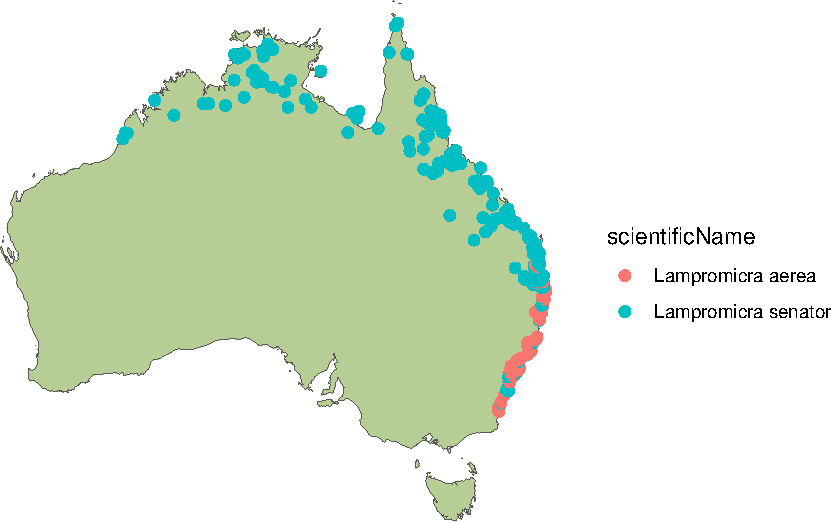
\includegraphics{./scope_files/figure-pdf/unnamed-chunk-1-1.pdf}

\hypertarget{spatial-scope}{%
\section{Spatial scope}\label{spatial-scope}}

Where the aim is to obtain data for targeted taxa in a given location.
In this case, the region name or area boundaries can be used to delimit
the area of interest. The example below shows all Insecta orders in the
state of Tasmania in Australia

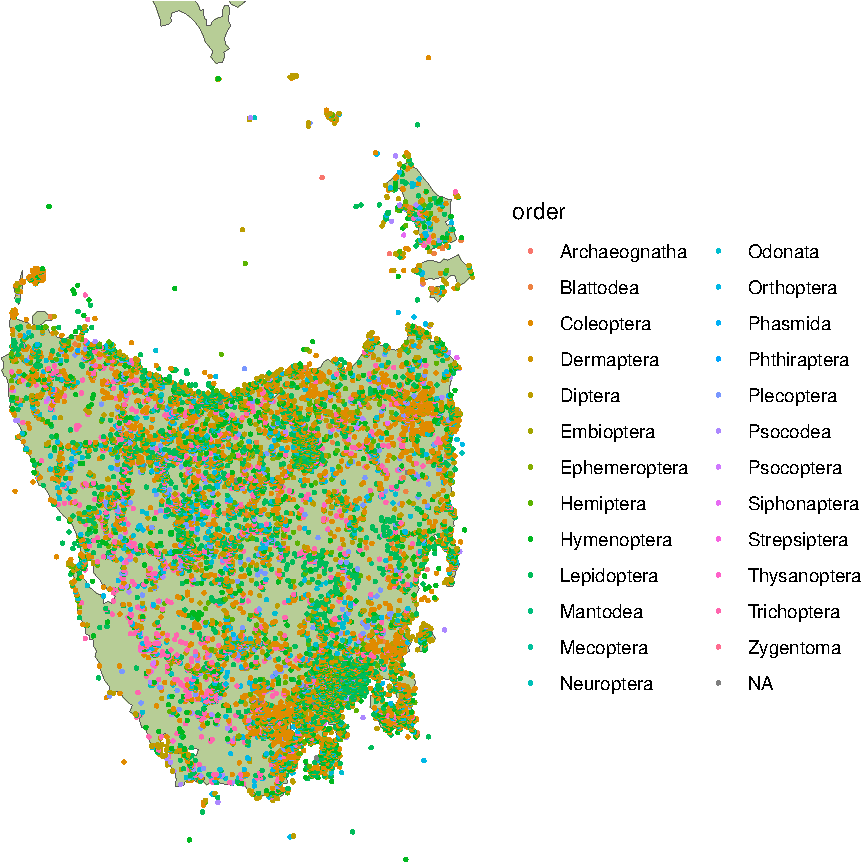
\includegraphics{./scope_files/figure-pdf/unnamed-chunk-2-1.pdf}

\bookmarksetup{startatroot}

\hypertarget{sec-download-data}{%
\chapter{Download occurrence data}\label{sec-download-data}}

Once you have decided on your data scope, we can precede to downloading
the data. We will introduce a few common data infrastructures that offer
open access biodiversity data and highlight some considerations when
choosing one in the context of your data scope. We will then discuss
some obstacles when consolidating data from multiple sources and the
importance of metadata.

\hypertarget{where-to-get-data-from}{%
\section{Where to get data from}\label{where-to-get-data-from}}

The \href{https://www.gbif.org/}{Global Biodiversity Information
Facility (GBIF)} network consists of a series of `node' organisations
who collate biodiversity data from their own countries, with GBIF acting
as an overarching organisation to store data from all nodes. Users that
are interested in obtaining data that has global coverage may want to
download directly from GBIF.

Alternatively, using a \emph{regional node} may be more relevant if your
project is at a smaller scale. For example, the
\href{www.ala.org.au}{Atlas of Living Australia (ALA)} is the Australian
node to GBIF and aggregates data from a broad range of providers such as
government initiatives, museums, and universities. Importantly, the ALA
uses their own taxonomic system and may vary with other data
infrastructures. To find other nodes, check out this
\href{https://www.gbif.org/the-gbif-network}{page}

If your project relates to citizen science then
\href{https://www.inaturalist.org/}{iNaturalist} may be a good option
for accessing crowd-sourced data of species observations.

\hypertarget{downloading-data}{%
\section{Downloading data}\label{downloading-data}}

Many developers have created R packages to interact with each data
infrastructures's API to aid access to biodiversity data. Here are a few
examples, we recommend taking a look at each package's documentation to
choose one that suits your project.

\begin{itemize}
\tightlist
\item
  \href{https://docs.ropensci.org/rgbif/}{\texttt{rgbif}} an interface
  to GBIF
\item
  \href{https://galah.ala.org.au/index.html}{\texttt{galah}} an
  interface to a number living Atlases, as well as GBIF
\item
  \href{https://docs.ropensci.org/rinat/}{\texttt{rinat}} an interface
  to iNaturalist observations
\item
  \href{https://docs.ropensci.org/rebird/}{\texttt{rebird}} an interface
  with the eBird webservices.
\item
  \href{https://docs.ropensci.org/spocc/}{\texttt{spocc}} a R package to
  query and collect species occurrence data from various sources
  including \href{https://github.com/ropensci/rvertnet}{VertNet},
  \href{http://www.idigbio.org/}{iDigBio} and others.
\end{itemize}

One benefit of using \texttt{galah} is that enables users to acquire not
only species occurrence records but also taxonomic information, or
associated media such as images or sounds. Below we have included some
code blocks for downloading occurrence data with \texttt{galah} from
GBIF and a Spain node.

\hypertarget{gbif-data-via-galah}{%
\subsection{\texorpdfstring{GBIF data via
\texttt{galah}}{GBIF data via galah}}\label{gbif-data-via-galah}}

First, we have to configure \texttt{galah}. This is where you supply
your account credentials and set the atlas to a particular region. See
\texttt{?galah\_config} for more configuration options. You can
\href{https://docs.ropensci.org/rgbif/articles/gbif_credentials.html}{save
these credentials} in your \texttt{.Renviron} so you don't have to enter
it explicitly in code.

We will be downloading all occurrences for the African Elephant from
GBIF. This may take a while as it is around 12,000 records. Once
downloaded, you can save the records locally in your desired format. For
larger downloads, we recommend saving the data as \texttt{parquets}
using \texttt{arrow::write\_parquet}

\begin{Shaded}
\begin{Highlighting}[]
\FunctionTok{galah\_config}\NormalTok{(}\AttributeTok{email =} \FunctionTok{Sys.getenv}\NormalTok{(}\StringTok{"ALA\_EMAIL"}\NormalTok{),}
             \AttributeTok{username =} \FunctionTok{Sys.getenv}\NormalTok{(}\StringTok{"GBIF\_USER"}\NormalTok{),}
             \AttributeTok{password =} \FunctionTok{Sys.getenv}\NormalTok{(}\StringTok{"GBIF\_PWD"}\NormalTok{),}
             \AttributeTok{atlas =} \StringTok{"Global"}\NormalTok{)}

\NormalTok{african\_ele }\OtherTok{\textless{}{-}} \FunctionTok{galah\_call}\NormalTok{() }\SpecialCharTok{\%\textgreater{}\%} 
  \FunctionTok{galah\_identify}\NormalTok{(}\StringTok{"Loxodonta africana"}\NormalTok{) }\SpecialCharTok{\%\textgreater{}\%} 
  \FunctionTok{atlas\_occurrences}\NormalTok{()}

\NormalTok{arrow}\SpecialCharTok{::}\FunctionTok{write\_parquet}\NormalTok{(african\_ele, }\StringTok{"data/gbif/elephant"}\NormalTok{)}
\end{Highlighting}
\end{Shaded}

\begin{verbatim}
# A tibble: 12,537 x 50
      gbifID datasetKey  occur~1 kingdom phylum class order family genus species
 *     <dbl> <chr>       <chr>   <chr>   <chr>  <chr> <chr> <chr>  <chr> <chr>  
 1 924537719 95f132fe-f~ 73e088~ Animal~ Chord~ Mamm~ Prob~ Eleph~ Loxo~ Loxodo~
 2 924537718 95f132fe-f~ 73e0ad~ Animal~ Chord~ Mamm~ Prob~ Eleph~ Loxo~ Loxodo~
 3 924537717 95f132fe-f~ 73f0f6~ Animal~ Chord~ Mamm~ Prob~ Eleph~ Loxo~ Loxodo~
 4 923926679 50c9509d-2~ http:/~ Animal~ Chord~ Mamm~ Prob~ Eleph~ Loxo~ Loxodo~
 5 923924124 50c9509d-2~ http:/~ Animal~ Chord~ Mamm~ Prob~ Eleph~ Loxo~ Loxodo~
 6 922237429 6ac3f774-d~ <NA>    Animal~ Chord~ Mamm~ Prob~ Eleph~ Loxo~ Loxodo~
 7 922237412 6ac3f774-d~ <NA>    Animal~ Chord~ Mamm~ Prob~ Eleph~ Loxo~ Loxodo~
 8 922237188 6ac3f774-d~ <NA>    Animal~ Chord~ Mamm~ Prob~ Eleph~ Loxo~ Loxodo~
 9 922237135 6ac3f774-d~ <NA>    Animal~ Chord~ Mamm~ Prob~ Eleph~ Loxo~ Loxodo~
10 922237121 6ac3f774-d~ <NA>    Animal~ Chord~ Mamm~ Prob~ Eleph~ Loxo~ Loxodo~
# ... with 12,527 more rows, 40 more variables: infraspecificEpithet <chr>,
#   taxonRank <chr>, scientificName <chr>, verbatimScientificName <chr>,
#   verbatimScientificNameAuthorship <chr>, countryCode <chr>, locality <chr>,
#   stateProvince <chr>, occurrenceStatus <chr>, individualCount <dbl>,
#   publishingOrgKey <chr>, decimalLatitude <dbl>, decimalLongitude <dbl>,
#   coordinateUncertaintyInMeters <dbl>, coordinatePrecision <dbl>,
#   elevation <dbl>, elevationAccuracy <dbl>, depth <dbl>, ...
\end{verbatim}

\hypertarget{regional-node-via-galah}{%
\subsection{\texorpdfstring{Regional node via
\texttt{galah}}{Regional node via galah}}\label{regional-node-via-galah}}

In order to access data from the Australia node, we will need to
reconfigure \texttt{galah} so that our query points to Australia. After
that, we will download all records for the Pink Robin.

\begin{Shaded}
\begin{Highlighting}[]
\FunctionTok{galah\_config}\NormalTok{(}\AttributeTok{email =} \FunctionTok{Sys.getenv}\NormalTok{(}\StringTok{"ALA\_EMAIL"}\NormalTok{), }
             \AttributeTok{atlas =} \StringTok{"Australia"}\NormalTok{)}

\NormalTok{pink\_robin }\OtherTok{\textless{}{-}} \FunctionTok{galah\_call}\NormalTok{() }\SpecialCharTok{\%\textgreater{}\%} 
  \FunctionTok{galah\_identify}\NormalTok{(}\StringTok{"Petroica rodinogaster"}\NormalTok{) }\SpecialCharTok{\%\textgreater{}\%} 
\NormalTok{  atlas\_occurrences}
\end{Highlighting}
\end{Shaded}

\begin{verbatim}
# A tibble: 11,992 x 8
   decimal~1 decim~2 eventDate           scien~3 taxon~4 recor~5 dataR~6 occur~7
 *     <dbl>   <dbl> <dttm>              <chr>   <chr>   <chr>   <chr>   <chr>  
 1     -43.7    146. NA                  Petroi~ https:~ 81d100~ Histor~ PRESENT
 2     -43.7    146. NA                  Petroi~ https:~ 235009~ Histor~ PRESENT
 3     -43.7    146. 1971-02-03 14:00:00 Petroi~ https:~ 0f644c~ Histor~ PRESENT
 4     -43.7    146. 2020-10-07 02:39:00 Petroi~ https:~ 77d610~ iNatur~ PRESENT
 5     -43.7    146. 2015-09-22 14:00:00 Petroi~ https:~ e92acb~ eBird ~ PRESENT
 6     -43.6    146. 2002-01-03 13:00:00 Petroi~ https:~ 1a4ac6~ BirdLi~ PRESENT
 7     -43.6    146. NA                  Petroi~ https:~ 28ec00~ Histor~ PRESENT
 8     -43.6    146. 2020-12-27 13:00:00 Petroi~ https:~ cbc68d~ eBird ~ PRESENT
 9     -43.6    146. 2021-03-07 13:00:00 Petroi~ https:~ 961160~ eBird ~ PRESENT
10     -43.6    146. 2020-12-26 13:00:00 Petroi~ https:~ 035bfb~ eBird ~ PRESENT
# ... with 11,982 more rows, and abbreviated variable names 1: decimalLatitude,
#   2: decimalLongitude, 3: scientificName, 4: taxonConceptID, 5: recordID,
#   6: dataResourceName, 7: occurrenceStatus
\end{verbatim}

\hypertarget{choosing-specific-data-columns}{%
\section{Choosing specific data
columns}\label{choosing-specific-data-columns}}

By default, \texttt{atlas\_occurrences} will return a tibble with a
selection of columns containing taxonomic and spatial data as well as
other metadata. Alternatively, you can use \texttt{galah\_select} to
subset the columns that are relevant for your work. To see all available
fields you can choose from:

\begin{Shaded}
\begin{Highlighting}[]
\FunctionTok{show\_all}\NormalTok{(fields) }
\end{Highlighting}
\end{Shaded}

\begin{verbatim}
# A tibble: 611 x 4
   id                    description                                 type  link 
   <chr>                 <chr>                                       <chr> <chr>
 1 abcdTypeStatus        ABCD field in use by herbaria               fiel~ <NA> 
 2 acceptedNameUsage     http://rs.tdwg.org/dwc/terms/acceptedNameU~ fiel~ <NA> 
 3 acceptedNameUsageID   http://rs.tdwg.org/dwc/terms/acceptedNameU~ fiel~ <NA> 
 4 accessRights          <NA>                                        fiel~ <NA> 
 5 assertionUserId       User ID of the person who has made an asse~ fiel~ <NA> 
 6 assertions            A list of all assertions (user and system ~ fiel~ <NA> 
 7 associatedMedia       http://rs.tdwg.org/dwc/terms/associatedMed~ fiel~ <NA> 
 8 associatedOccurrences http://rs.tdwg.org/dwc/terms/associatedOcc~ fiel~ <NA> 
 9 associatedOrganisms   http://rs.tdwg.org/dwc/terms/associatedOrg~ fiel~ <NA> 
10 associatedReferences  http://rs.tdwg.org/dwc/terms/associatedRef~ fiel~ <NA> 
# ... with 601 more rows
\end{verbatim}

Here, we will choose a smaller subsets of 8 columns to download for the
Pink Robin

\begin{Shaded}
\begin{Highlighting}[]
\NormalTok{project\_fields }\OtherTok{\textless{}{-}} \FunctionTok{c}\NormalTok{(}\StringTok{"recordID"}\NormalTok{,}
                    \StringTok{"eventDate"}\NormalTok{,}
                    \StringTok{"year"}\NormalTok{, }
                    \StringTok{"basisOfRecord"}\NormalTok{, }
                    \StringTok{"occurrenceStatus"}\NormalTok{,}
                    \StringTok{"scientificName"}\NormalTok{,}
                    \StringTok{"decimalLatitude"}\NormalTok{,}
                    \StringTok{"decimalLongitude"}\NormalTok{)}

\NormalTok{pink\_robin\_projfields }\OtherTok{\textless{}{-}} \FunctionTok{galah\_call}\NormalTok{() }\SpecialCharTok{\%\textgreater{}\%} 
  \FunctionTok{galah\_identify}\NormalTok{(}\StringTok{"Petroica rodinogaster"}\NormalTok{) }\SpecialCharTok{\%\textgreater{}\%} 
  \FunctionTok{galah\_select}\NormalTok{(project\_fields) }\SpecialCharTok{\%\textgreater{}\%} 
  \FunctionTok{atlas\_occurrences}\NormalTok{()}
\end{Highlighting}
\end{Shaded}

\begin{verbatim}
# A tibble: 11,992 x 8
   recordID    eventDate            year basis~1 occur~2 scien~3 decim~4 decim~5
 * <chr>       <dttm>              <dbl> <chr>   <chr>   <chr>     <dbl>   <dbl>
 1 000fc2ef-b~ 1976-12-18 13:00:00  1976 HUMAN_~ PRESENT Petroi~   -37.4    144.
 2 001410fd-3~ 1978-05-23 14:00:00  1978 HUMAN_~ PRESENT Petroi~   -38.2    142.
 3 00164a76-0~ 1977-12-15 13:00:00  1977 HUMAN_~ PRESENT Petroi~   -42.9    147.
 4 001bfca5-4~ 1940-12-31 14:00:00  1941 OBSERV~ PRESENT Petroi~   -36.4    147.
 5 001e33bd-b~ 2002-10-17 14:00:00  2002 HUMAN_~ PRESENT Petroi~   -40.9    146.
 6 0021cc7c-a~ 2016-04-09 14:00:00  2016 OCCURR~ PRESENT Petroi~   -38.6    144.
 7 00287e24-8~ 2021-01-14 13:00:00  2021 HUMAN_~ PRESENT Petroi~   -37.5    146.
 8 002e05a7-b~ 2000-07-24 14:00:00  2000 OBSERV~ PRESENT Petroi~   -38.4    145.
 9 00327fc2-a~ 1983-11-23 13:00:00  1983 PRESER~ PRESENT Petroi~   -37.3    149.
10 0035016f-a~ NA                     NA HUMAN_~ PRESENT Petroi~   -41.1    146.
# ... with 11,982 more rows, and abbreviated variable names 1: basisOfRecord,
#   2: occurrenceStatus, 3: scientificName, 4: decimalLatitude,
#   5: decimalLongitude
\end{verbatim}

\hypertarget{refining-your-data-download}{%
\section{Refining your data
download}\label{refining-your-data-download}}

Open access biodiversity data comes from many different providers such
as universities, research institutes (museums and herbariums),
government and the general public. As such, data type and quality can
vary considerably. For example, museums harbour older records that are
associated with a preserved specimen, whereas citizen sourced data are
often images captured from a smart phone.

Refining your download query ensures higher quality data and also
reduces the download size as many data infrastructures impose
constraints to download size. Below we have illustrated how you can
refine your query a few quality measures using \texttt{galah\_filter}.

\hypertarget{by-year}{%
\subsubsection{By Year}\label{by-year}}

Generally, old data records tend to be insufficient or less reliable as
taxonomic knowledge and GPS tools were not readily available. For this
reason, many users consider removing all occurrence records before a
certain year to increase data precision (Gueta and Carmel 2016; J. R.
Marsh et al. 2022) .

Choosing the year `cut-off' is relatively arbitary, but the most
commonly used year is 1945 (Zizka et al. 2020a; Führding-Potschkat,
Kreft, and Ickert-Bond 2022), although some studies discard all data
collected before 1990 (Gueta and Carmel 2016; J. R. Marsh et al. 2022).

Here we will narrow the Pink Robin query from above to records after
1945 using \texttt{galah\_filter}:

\begin{Shaded}
\begin{Highlighting}[]
\NormalTok{pink\_robin\_post1945 }\OtherTok{\textless{}{-}} \FunctionTok{galah\_call}\NormalTok{() }\SpecialCharTok{\%\textgreater{}\%} 
  \FunctionTok{galah\_identify}\NormalTok{(}\StringTok{"Petroica rodinogaster"}\NormalTok{) }\SpecialCharTok{\%\textgreater{}\%} 
  \FunctionTok{galah\_filter}\NormalTok{(year }\SpecialCharTok{\textgreater{}} \DecValTok{1945}\NormalTok{) }\SpecialCharTok{\%\textgreater{}\%} 
  \FunctionTok{atlas\_occurrences}\NormalTok{()}
\end{Highlighting}
\end{Shaded}

\hypertarget{basis-of-record}{%
\subsubsection{Basis of record}\label{basis-of-record}}

Basis of record is a
\href{https://dwc.tdwg.org/terms/\#dwc:basisOfRecord}{Darwin Core term}
that refers to the specific nature of the occurrence record. It can be
used to refine your data download and ensure consistency when
consolidating data from multiple organisations (Führding-Potschkat,
Kreft, and Ickert-Bond 2022).

There are 6 different classes for basis of record:

\begin{itemize}
\tightlist
\item
  Living Specimen - a specimen that is alive, e.g.~a living plant in a
  national park
\item
  Preserved Specimen - a specimen that has been preserved, for example,
  a dried plant on an herbarium sheet
\item
  Fossil Specimen - a preserved specimen that is a fossil
\item
  Material Sample - a genetic or environmental sample
\item
  Material Citation - A reference to, or citation of, a specimen in
  scholarly publications, e.g a citation of a physical specimen in a
  scientific journal
\item
  Human Observation - an output of human observation process
  e.g.~evidence of an occurrence taken from field notes or an occurrence
  without any physical evidence
\item
  Machine Observation - An output of a machine observation process
  e.g.~a photograph, a video, an audio recording, a remote sensing image
  or an occurrence record based on telemetry.
\end{itemize}

Depending on your data scope, it may be practical to limit data that can
be traced to a physical specimen or observation (Godfree et al. 2021),
which we do for the Pink Robin below

\begin{Shaded}
\begin{Highlighting}[]
\NormalTok{tractable\_records }\OtherTok{\textless{}{-}} \FunctionTok{c}\NormalTok{(}\StringTok{"LIVING\_SPECIMEN"}\NormalTok{, }
                       \StringTok{"PRESERVED\_SPECIMEN"}\NormalTok{, }
                       \StringTok{"MATERIAL\_SAMPLE"}\NormalTok{, }
                       \StringTok{"MACHINE\_OBSERVATION"}\NormalTok{)}

\NormalTok{pink\_robin\_tractable }\OtherTok{\textless{}{-}} \FunctionTok{galah\_call}\NormalTok{() }\SpecialCharTok{\%\textgreater{}\%} 
  \FunctionTok{galah\_identify}\NormalTok{(}\StringTok{"Petroica rodinogaster"}\NormalTok{) }\SpecialCharTok{\%\textgreater{}\%} 
  \FunctionTok{galah\_filter}\NormalTok{(basisOfRecord }\SpecialCharTok{==}\NormalTok{ tractable\_records) }\SpecialCharTok{\%\textgreater{}\%} 
  \FunctionTok{atlas\_occurrences}\NormalTok{()}
\end{Highlighting}
\end{Shaded}

\hypertarget{assertions}{%
\subsubsection{Assertions}\label{assertions}}

Data infrastructures use assertions to internally grade the quality,
completeness and consistency of each occurrence record. Assertions take
values of either 1 or 0, indicating the presence or absence of the data
quality issue. Note that assertions may vary depending what atlas you
have configured to. You can see the available assertions and their
descriptions using:

\begin{Shaded}
\begin{Highlighting}[]
\FunctionTok{show\_all}\NormalTok{(}\StringTok{"assertions"}\NormalTok{) }
\end{Highlighting}
\end{Shaded}

\begin{verbatim}
# A tibble: 117 x 4
   id                                 description                  categ~1 type 
   <chr>                              <chr>                        <chr>   <chr>
 1 AMBIGUOUS_COLLECTION               Ambiguous collection         Warning asse~
 2 AMBIGUOUS_INSTITUTION              Ambiguous institution        Warning asse~
 3 BASIS_OF_RECORD_INVALID            Basis of record badly formed Warning asse~
 4 biosecurityIssue                   Biosecurity issue            Error   asse~
 5 COLLECTION_MATCH_FUZZY             Collection match fuzzy       Warning asse~
 6 COLLECTION_MATCH_NONE              Collection not matched       Warning asse~
 7 CONTINENT_COUNTRY_MISMATCH         Continent country mismatch   Warning asse~
 8 CONTINENT_DERIVED_FROM_COORDINATES Continent derived from coor~ Warning asse~
 9 CONTINENT_INVALID                  Continent invalid            Warning asse~
10 COORDINATE_ACCURACY_INVALID        Coordinate accuracy invalid  Warning asse~
# ... with 107 more rows, and abbreviated variable name 1: category
\end{verbatim}

Once you have decided which assertions are important for your project
you can further refine your download.

\bookmarksetup{startatroot}

\hypertarget{precleaning}{%
\chapter{Precleaning}\label{precleaning}}

Precleaning prepares the dataset in a general manner so that it is
formatted in a logical and consistent manner. It is a `broad sweep'
procedure that allows you to familiarise with the data but it also makes
the next stage of in-depth data cleaning proceed more smoothly
(streamdna 2020). We will discuss some approaches on how to be curious
with your data and how to detect and handle string inconsistencies,
missing data and outliers.

\hypertarget{metadata}{%
\section{Metadata}\label{metadata}}

Metadata describes your dataset. It defines each variable and describes
its contents such as what units a variable is measured in. Data
infrastructures that uses Darwin Core terms will have interoperable
metadata. All Darwin Core term definitions can be found
\href{https://dwc.tdwg.org/terms/}{here}, we suggest using
\texttt{Ctrl/CMD\ F} and searching your variable name on the
\href{https://dwc.tdwg.org/terms/}{webpage}. Don't hesitate to Google
variable names if you are unsure what they represent.

\hypertarget{initial-inspection}{%
\section{Initial inspection}\label{initial-inspection}}

A great way to get an initial overview of your data is to use the R
package \texttt{skimr}. Importantly \texttt{skimr} produces tables of
descriptive statistics, such as amount of missing data, for every
variable

The output is also grouped by data type (numeric, character, date) so
you can also check for any inconsistencies. As you are looking through
the output, ask yourself whether the data is in line with your
expectation. If you requested data for a group of species, are they all
represented? Are the values for a variable reasonable? Looking at the
quartiles will help you get the sense of the distribution of data. These
considerations will help you detect potential issues in the data.

\begin{Shaded}
\begin{Highlighting}[]
\FunctionTok{library}\NormalTok{(skimr)}

\FunctionTok{skim}\NormalTok{(african\_ele)}
\end{Highlighting}
\end{Shaded}

Here is the \texttt{skimr} report for our African elephant dataset we
\protect\hyperlink{sec-download-data}{downloaded earlier}

\begin{longtable}[]{@{}ll@{}}
\caption{Data summary}\tabularnewline
\toprule()
\endhead
Name & african\_ele \\
Number of rows & 12537 \\
Number of columns & 50 \\
\_\_\_\_\_\_\_\_\_\_\_\_\_\_\_\_\_\_\_\_\_\_\_ & \\
Column type frequency: & \\
character & 31 \\
logical & 1 \\
numeric & 15 \\
POSIXct & 3 \\
\_\_\_\_\_\_\_\_\_\_\_\_\_\_\_\_\_\_\_\_\_\_\_\_ & \\
Group variables & None \\
\bottomrule()
\end{longtable}

\textbf{Variable type: character}

\begin{longtable}[]{@{}
  >{\raggedright\arraybackslash}p{(\columnwidth - 14\tabcolsep) * \real{0.3626}}
  >{\raggedleft\arraybackslash}p{(\columnwidth - 14\tabcolsep) * \real{0.1099}}
  >{\raggedleft\arraybackslash}p{(\columnwidth - 14\tabcolsep) * \real{0.1538}}
  >{\raggedleft\arraybackslash}p{(\columnwidth - 14\tabcolsep) * \real{0.0440}}
  >{\raggedleft\arraybackslash}p{(\columnwidth - 14\tabcolsep) * \real{0.0440}}
  >{\raggedleft\arraybackslash}p{(\columnwidth - 14\tabcolsep) * \real{0.0659}}
  >{\raggedleft\arraybackslash}p{(\columnwidth - 14\tabcolsep) * \real{0.0989}}
  >{\raggedleft\arraybackslash}p{(\columnwidth - 14\tabcolsep) * \real{0.1209}}@{}}
\toprule()
\begin{minipage}[b]{\linewidth}\raggedright
skim\_variable
\end{minipage} & \begin{minipage}[b]{\linewidth}\raggedleft
n\_missing
\end{minipage} & \begin{minipage}[b]{\linewidth}\raggedleft
complete\_rate
\end{minipage} & \begin{minipage}[b]{\linewidth}\raggedleft
min
\end{minipage} & \begin{minipage}[b]{\linewidth}\raggedleft
max
\end{minipage} & \begin{minipage}[b]{\linewidth}\raggedleft
empty
\end{minipage} & \begin{minipage}[b]{\linewidth}\raggedleft
n\_unique
\end{minipage} & \begin{minipage}[b]{\linewidth}\raggedleft
whitespace
\end{minipage} \\
\midrule()
\endhead
datasetKey & 0 & 1.00 & 36 & 36 & 0 & 132 & 0 \\
occurrenceID & 708 & 0.94 & 1 & 81 & 0 & 11787 & 0 \\
kingdom & 0 & 1.00 & 8 & 8 & 0 & 1 & 0 \\
phylum & 0 & 1.00 & 8 & 8 & 0 & 1 & 0 \\
class & 0 & 1.00 & 8 & 8 & 0 & 1 & 0 \\
order & 0 & 1.00 & 11 & 11 & 0 & 1 & 0 \\
family & 0 & 1.00 & 12 & 12 & 0 & 1 & 0 \\
genus & 0 & 1.00 & 9 & 9 & 0 & 1 & 0 \\
species & 0 & 1.00 & 18 & 18 & 0 & 1 & 0 \\
infraspecificEpithet & 12410 & 0.01 & 8 & 13 & 0 & 2 & 0 \\
taxonRank & 0 & 1.00 & 7 & 10 & 0 & 3 & 0 \\
scientificName & 0 & 1.00 & 12 & 37 & 0 & 5 & 0 \\
verbatimScientificName & 3 & 1.00 & 12 & 53 & 0 & 32 & 0 \\
verbatimScientificNameAuthorship & 10964 & 0.13 & 2 & 31 & 0 & 255 &
0 \\
countryCode & 1461 & 0.88 & 2 & 2 & 0 & 44 & 0 \\
locality & 9211 & 0.27 & 3 & 254 & 0 & 686 & 0 \\
stateProvince & 3573 & 0.72 & 3 & 43 & 0 & 182 & 0 \\
occurrenceStatus & 0 & 1.00 & 6 & 7 & 0 & 2 & 0 \\
publishingOrgKey & 0 & 1.00 & 36 & 36 & 0 & 102 & 0 \\
basisOfRecord & 0 & 1.00 & 10 & 19 & 0 & 9 & 0 \\
institutionCode & 1325 & 0.89 & 2 & 76 & 0 & 103 & 0 \\
collectionCode & 1353 & 0.89 & 1 & 41 & 0 & 164 & 0 \\
catalogNumber & 1553 & 0.88 & 1 & 36 & 0 & 10866 & 0 \\
recordNumber & 12420 & 0.01 & 1 & 37 & 0 & 77 & 0 \\
identifiedBy & 4646 & 0.63 & 2 & 81 & 0 & 1464 & 0 \\
license & 0 & 1.00 & 7 & 12 & 0 & 3 & 0 \\
rightsHolder & 4240 & 0.66 & 2 & 56 & 0 & 1634 & 0 \\
recordedBy & 2138 & 0.83 & 1 & 160 & 0 & 1972 & 0 \\
establishmentMeans & 12249 & 0.02 & 6 & 6 & 0 & 1 & 0 \\
mediaType & 5021 & 0.60 & 5 & 16 & 0 & 4 & 0 \\
issue & 397 & 0.97 & 15 & 191 & 0 & 130 & 0 \\
\bottomrule()
\end{longtable}

\textbf{Variable type: logical}

\begin{longtable}[]{@{}lrrrl@{}}
\toprule()
skim\_variable & n\_missing & complete\_rate & mean & count \\
\midrule()
\endhead
typeStatus & 12537 & 0 & NaN & : \\
\bottomrule()
\end{longtable}

\textbf{Variable type: numeric}

\begin{longtable}[]{@{}
  >{\raggedright\arraybackslash}p{(\columnwidth - 20\tabcolsep) * \real{0.1961}}
  >{\raggedleft\arraybackslash}p{(\columnwidth - 20\tabcolsep) * \real{0.0654}}
  >{\raggedleft\arraybackslash}p{(\columnwidth - 20\tabcolsep) * \real{0.0915}}
  >{\raggedleft\arraybackslash}p{(\columnwidth - 20\tabcolsep) * \real{0.0915}}
  >{\raggedleft\arraybackslash}p{(\columnwidth - 20\tabcolsep) * \real{0.0850}}
  >{\raggedleft\arraybackslash}p{(\columnwidth - 20\tabcolsep) * \real{0.0784}}
  >{\raggedleft\arraybackslash}p{(\columnwidth - 20\tabcolsep) * \real{0.0915}}
  >{\raggedleft\arraybackslash}p{(\columnwidth - 20\tabcolsep) * \real{0.0915}}
  >{\raggedleft\arraybackslash}p{(\columnwidth - 20\tabcolsep) * \real{0.0850}}
  >{\raggedleft\arraybackslash}p{(\columnwidth - 20\tabcolsep) * \real{0.0850}}
  >{\raggedright\arraybackslash}p{(\columnwidth - 20\tabcolsep) * \real{0.0392}}@{}}
\toprule()
\begin{minipage}[b]{\linewidth}\raggedright
skim\_variable
\end{minipage} & \begin{minipage}[b]{\linewidth}\raggedleft
n\_missing
\end{minipage} & \begin{minipage}[b]{\linewidth}\raggedleft
complete\_rate
\end{minipage} & \begin{minipage}[b]{\linewidth}\raggedleft
mean
\end{minipage} & \begin{minipage}[b]{\linewidth}\raggedleft
sd
\end{minipage} & \begin{minipage}[b]{\linewidth}\raggedleft
p0
\end{minipage} & \begin{minipage}[b]{\linewidth}\raggedleft
p25
\end{minipage} & \begin{minipage}[b]{\linewidth}\raggedleft
p50
\end{minipage} & \begin{minipage}[b]{\linewidth}\raggedleft
p75
\end{minipage} & \begin{minipage}[b]{\linewidth}\raggedleft
p100
\end{minipage} & \begin{minipage}[b]{\linewidth}\raggedright
hist
\end{minipage} \\
\midrule()
\endhead
gbifID & 0 & 1.00 & 2535815516.94 & 960444243.67 & 49926810.00 &
1802649142.00 & 2465251941.00 & 3.351048e+09 & 4.029318e+09 & ▁▅▇▅▇ \\
individualCount & 10226 & 0.18 & 4.81 & 14.03 & 0.00 & 1.00 & 1.00 &
2.000000e+00 & 2.920000e+02 & ▇▁▁▁▁ \\
decimalLatitude & 1350 & 0.89 & -10.01 & 14.67 & -34.58 & -24.06 & -6.25
& 4.800000e-01 & 5.215000e+01 & ▇▅▅▁▁ \\
decimalLongitude & 1350 & 0.89 & 25.56 & 12.35 & -122.33 & 22.97 & 31.08
& 3.480000e+01 & 4.053000e+01 & ▁▁▁▂▇ \\
coordinateUncertaintyInMeters & 3966 & 0.68 & 41636.59 & 158053.45 &
1.00 & 29775.00 & 30580.00 & 3.142200e+04 & 5.635548e+06 & ▇▁▁▁▁ \\
coordinatePrecision & 12512 & 0.00 & 0.00 & 0.00 & 0.00 & 0.00 & 0.00 &
0.000000e+00 & 0.000000e+00 & ▁▁▁▁▇ \\
elevation & 12501 & 0.00 & 154.42 & 421.59 & 0.00 & 0.00 & 0.00 &
1.375000e+01 & 2.134000e+03 & ▇▁▁▁▁ \\
elevationAccuracy & 12507 & 0.00 & 0.83 & 3.73 & 0.00 & 0.00 & 0.00 &
0.000000e+00 & 2.000000e+01 & ▇▁▁▁▁ \\
depth & 12509 & 0.00 & 0.00 & 0.00 & 0.00 & 0.00 & 0.00 & 0.000000e+00 &
0.000000e+00 & ▁▁▇▁▁ \\
depthAccuracy & 12509 & 0.00 & 0.00 & 0.00 & 0.00 & 0.00 & 0.00 &
0.000000e+00 & 0.000000e+00 & ▁▁▇▁▁ \\
day & 1254 & 0.90 & 16.27 & 8.74 & 1.00 & 9.00 & 17.00 & 2.400000e+01 &
3.100000e+01 & ▇▆▇▇▇ \\
month & 1191 & 0.91 & 6.92 & 3.33 & 1.00 & 4.00 & 7.00 & 1.000000e+01 &
1.200000e+01 & ▆▅▅▇▇ \\
year & 997 & 0.92 & 2011.05 & 19.34 & 1799.00 & 2011.00 & 2016.00 &
2.019000e+03 & 2.023000e+03 & ▁▁▁▁▇ \\
taxonKey & 0 & 1.00 & 2517047.48 & 747546.46 & 2435350.00 & 2435350.00 &
2435350.00 & 2.435350e+06 & 1.150335e+07 & ▇▁▁▁▁ \\
speciesKey & 0 & 1.00 & 2435350.00 & 0.00 & 2435350.00 & 2435350.00 &
2435350.00 & 2.435350e+06 & 2.435350e+06 & ▁▁▇▁▁ \\
\bottomrule()
\end{longtable}

\textbf{Variable type: POSIXct}

\begin{longtable}[]{@{}
  >{\raggedright\arraybackslash}p{(\columnwidth - 12\tabcolsep) * \real{0.1468}}
  >{\raggedleft\arraybackslash}p{(\columnwidth - 12\tabcolsep) * \real{0.0917}}
  >{\raggedleft\arraybackslash}p{(\columnwidth - 12\tabcolsep) * \real{0.1284}}
  >{\raggedright\arraybackslash}p{(\columnwidth - 12\tabcolsep) * \real{0.1835}}
  >{\raggedright\arraybackslash}p{(\columnwidth - 12\tabcolsep) * \real{0.1835}}
  >{\raggedright\arraybackslash}p{(\columnwidth - 12\tabcolsep) * \real{0.1835}}
  >{\raggedleft\arraybackslash}p{(\columnwidth - 12\tabcolsep) * \real{0.0826}}@{}}
\toprule()
\begin{minipage}[b]{\linewidth}\raggedright
skim\_variable
\end{minipage} & \begin{minipage}[b]{\linewidth}\raggedleft
n\_missing
\end{minipage} & \begin{minipage}[b]{\linewidth}\raggedleft
complete\_rate
\end{minipage} & \begin{minipage}[b]{\linewidth}\raggedright
min
\end{minipage} & \begin{minipage}[b]{\linewidth}\raggedright
max
\end{minipage} & \begin{minipage}[b]{\linewidth}\raggedright
median
\end{minipage} & \begin{minipage}[b]{\linewidth}\raggedleft
n\_unique
\end{minipage} \\
\midrule()
\endhead
eventDate & 997 & 0.92 & 1799-01-01 00:00:00 & 2023-02-07 09:17:14 &
2016-02-07 12:00:00 & 8324 \\
dateIdentified & 4150 & 0.67 & 1783-01-01 00:00:00 & 2023-02-07 21:51:36
& 2020-04-16 19:35:25 & 7242 \\
lastInterpreted & 0 & 1.00 & 2023-01-24 14:57:46 & 2023-02-14 01:52:09 &
2023-02-13 16:01:27 & 10885 \\
\bottomrule()
\end{longtable}

\hypertarget{string-inconsistencies}{%
\section{String inconsistencies}\label{string-inconsistencies}}

String inconsistencies include mispellings, capitalisation errors,
misplaced punctuations or trailing white spaces. We will use the
\texttt{janitor} R package to explore whether our data has any of these
issues. The function \texttt{tably} will compute a counts and percent of
total rows for each unique value.

We recommend \texttt{tabyl-ing} any character strings that are relevant
to your project. For example, here is the
\href{https://dwc.tdwg.org/terms/\#dwc:stateProvince}{\texttt{stateProvince}}
in alphabetical order.

\begin{Shaded}
\begin{Highlighting}[]
\FunctionTok{library}\NormalTok{(janitor)}

\NormalTok{african\_ele }\SpecialCharTok{\%\textgreater{}\%}
  \FunctionTok{pull}\NormalTok{(stateProvince) }\SpecialCharTok{\%\textgreater{}\%} 
  \FunctionTok{tabyl}\NormalTok{() }\SpecialCharTok{\%\textgreater{}\%} 
  \FunctionTok{tibble}\NormalTok{() }\SpecialCharTok{\%\textgreater{}\%} 
  \FunctionTok{print}\NormalTok{(}\AttributeTok{n =} \DecValTok{20}\NormalTok{)}
\end{Highlighting}
\end{Shaded}

\begin{verbatim}
# A tibble: 183 x 4
   .                     n   percent valid_percent
   <chr>             <int>     <dbl>         <dbl>
 1 Agadez                1 0.0000798      0.000112
 2 Al Qahirah            1 0.0000798      0.000112
 3 Alibori             601 0.0479         0.0670  
 4 Arusha              231 0.0184         0.0258  
 5 Arusha Region         1 0.0000798      0.000112
 6 Atacora             366 0.0292         0.0408  
 7 Atakora             239 0.0191         0.0267  
 8 Balaka                7 0.000558       0.000781
 9 Bassila               1 0.0000798      0.000112
10 Batha                 1 0.0000798      0.000112
11 Bauchi                3 0.000239       0.000335
12 Bengo                 3 0.000239       0.000335
13 Borgou                7 0.000558       0.000781
14 Budongo Forest        1 0.0000798      0.000112
15 Bushenyi             61 0.00487        0.00680 
16 Cabo Delgado          2 0.000160       0.000223
17 Cape Prov.            2 0.000160       0.000223
18 Cape Province         1 0.0000798      0.000112
19 Central             113 0.00901        0.0126  
20 Central Equatoria     2 0.000160       0.000223
# ... with 163 more rows
\end{verbatim}

From the \texttt{tabyl} output, we can see there are few different
variations of \texttt{Province}, \texttt{Prov.}, \texttt{Prov}. As an
example, we will correct these with the \texttt{tidyverse} packages
\texttt{stringr}, \texttt{dplyr}, \texttt{tidyr} as well as
\texttt{glue}. If you are not very familiar with regular expressions, we
highly recommend this
\href{https://evoldyn.gitlab.io/evomics-2018/ref-sheets/R_strings.pdf}{cheatsheet}

\begin{Shaded}
\begin{Highlighting}[]
\FunctionTok{library}\NormalTok{(tidyverse)}
\FunctionTok{library}\NormalTok{(glue)}

\CommentTok{\# Create a regular expression to match Prov. and Prov}
\CommentTok{\# The pattern below means Prov that is NOT followed by any lowercase letters}
\NormalTok{pattern }\OtherTok{=} \FunctionTok{regex}\NormalTok{(}\StringTok{"Prov(?![:lower:])"}\NormalTok{)}

\CommentTok{\# Use \textasciigrave{}str\_subset\textasciigrave{} to pull out the cases that match our pattern}
\CommentTok{\# Confirm that these are the problematic ones}
\CommentTok{\# Assign these into an object}
\FunctionTok{str\_subset}\NormalTok{(african\_ele}\SpecialCharTok{$}\NormalTok{stateProvince, }\AttributeTok{pattern =}\NormalTok{ pattern)}
\end{Highlighting}
\end{Shaded}

\begin{verbatim}
 [1] "Cape Prov."        "Cape Prov."        "West Nile Prov."  
 [4] "Central Prov"      "Central Prov"      "Coastal Prov"     
 [7] "Northeastern Prov" "Central Prov"      "Eastern Prov"     
[10] "Coastal Prov"     
\end{verbatim}

\begin{Shaded}
\begin{Highlighting}[]
\NormalTok{typos\_provinces }\OtherTok{\textless{}{-}} \FunctionTok{str\_subset}\NormalTok{(african\_ele}\SpecialCharTok{$}\NormalTok{stateProvince, }\AttributeTok{pattern =}\NormalTok{ pattern)}

\CommentTok{\# Create a new variable \textasciigrave{}stateProvince\_clean\textasciigrave{} using \textasciigrave{}mutate\textasciigrave{}, \textasciigrave{}if\_else\textasciigrave{}, \textasciigrave{}str\_detect\textasciigrave{} and \textasciigrave{}glue\textasciigrave{}}
\CommentTok{\# \textasciigrave{}str\_detect\textasciigrave{} will evaluate values of \textasciigrave{}stateProvince\textasciigrave{} that matches our pattern we defined earlier.}
\CommentTok{\# Matches will return TRUE, non{-}matches will return FALSE. }
\CommentTok{\# The \textasciigrave{}if\_else\textasciigrave{} will then evaluate these logicals (TRUE/FALSE/NA) }
\CommentTok{\# for TRUE values, the \textasciigrave{}glue\textasciigrave{} function will take the first part of the province name enclosed in and join it with word Province.}
\CommentTok{\# for FALSE values , it will just take the corresponding value in stateProvince}
\CommentTok{\# Note that we are assigning these changes to a new object (\textasciigrave{}african\_ele\_2\textasciigrave{})}
\NormalTok{african\_ele\_2 }\OtherTok{\textless{}{-}}\NormalTok{ african\_ele }\SpecialCharTok{\%\textgreater{}\%} 
  \FunctionTok{mutate}\NormalTok{(}\AttributeTok{stateProvince\_clean =} \FunctionTok{if\_else}\NormalTok{(}\FunctionTok{str\_detect}\NormalTok{(stateProvince, }\AttributeTok{pattern =}\NormalTok{ pattern),}
                                      \AttributeTok{true =} \FunctionTok{glue}\NormalTok{(}\StringTok{\textquotesingle{}\{word(stateProvince, sep = " P")\} Province\textquotesingle{}}\NormalTok{),}
                                      \AttributeTok{false =}\NormalTok{ stateProvince)}
\NormalTok{         ) }

\CommentTok{\# Once we\textquotesingle{}ve made the correction we want to check we\textquotesingle{}ve done it correctly.}
\CommentTok{\# ALWAYS CHECK YOUR CORRECTIONS}
\CommentTok{\# Use the \textasciigrave{}select\textasciigrave{} function to isolate columns that \textasciigrave{}starts\_with\textasciigrave{} "stateProvince"}
\CommentTok{\# Use the \textasciigrave{}filter\textasciigrave{} function to subset our the problematic provinces }
\NormalTok{african\_ele\_2 }\SpecialCharTok{\%\textgreater{}\%} 
  \FunctionTok{select}\NormalTok{(}\FunctionTok{starts\_with}\NormalTok{(}\StringTok{"stateProvince"}\NormalTok{)) }\SpecialCharTok{\%\textgreater{}\%} 
  \FunctionTok{filter}\NormalTok{(stateProvince }\SpecialCharTok{\%in\%}\NormalTok{ typos\_provinces)}
\end{Highlighting}
\end{Shaded}

\begin{verbatim}
# A tibble: 10 x 2
   stateProvince     stateProvince_clean  
   <chr>             <glue>               
 1 Cape Prov.        Cape Province        
 2 Cape Prov.        Cape Province        
 3 West Nile Prov.   West Nile Province   
 4 Central Prov      Central Province     
 5 Central Prov      Central Province     
 6 Coastal Prov      Coastal Province     
 7 Northeastern Prov Northeastern Province
 8 Central Prov      Central Province     
 9 Eastern Prov      Eastern Province     
10 Coastal Prov      Coastal Province     
\end{verbatim}

\begin{Shaded}
\begin{Highlighting}[]
\CommentTok{\# Its good practice to check the other values were not affected by your corrections}
\CommentTok{\# Here we are removing the NA with \textasciigrave{}drop\_na\textasciigrave{} and subsetting unique rows with \textasciigrave{}distinct\textasciigrave{}}
\NormalTok{african\_ele\_2 }\SpecialCharTok{\%\textgreater{}\%} 
  \FunctionTok{select}\NormalTok{(}\FunctionTok{starts\_with}\NormalTok{(}\StringTok{"stateProvince"}\NormalTok{)) }\SpecialCharTok{\%\textgreater{}\%} 
  \FunctionTok{drop\_na}\NormalTok{() }\SpecialCharTok{\%\textgreater{}\%} 
  \FunctionTok{distinct}\NormalTok{() }
\end{Highlighting}
\end{Shaded}

\begin{verbatim}
# A tibble: 182 x 2
   stateProvince    stateProvince_clean
   <chr>            <glue>             
 1 Southern         Southern           
 2 Taita Taveta     Taita Taveta       
 3 Mara             Mara               
 4 Arusha           Arusha             
 5 Simiyu           Simiyu             
 6 Morogoro         Morogoro           
 7 Mashonaland West Mashonaland West   
 8 Mpumalanga       Mpumalanga         
 9 KwaZulu-Natal    KwaZulu-Natal      
10 Manicaland       Manicaland         
# ... with 172 more rows
\end{verbatim}

\begin{Shaded}
\begin{Highlighting}[]
\CommentTok{\# Final check}
\CommentTok{\# Check with the original code that detected the issue}
\NormalTok{african\_ele\_2 }\SpecialCharTok{\%\textgreater{}\%}
  \FunctionTok{pull}\NormalTok{(stateProvince\_clean) }\SpecialCharTok{\%\textgreater{}\%} 
  \FunctionTok{tabyl}\NormalTok{() }\SpecialCharTok{\%\textgreater{}\%} 
  \FunctionTok{tibble}\NormalTok{() }\SpecialCharTok{\%\textgreater{}\%} 
  \FunctionTok{print}\NormalTok{(}\AttributeTok{n =} \DecValTok{20}\NormalTok{)}
\end{Highlighting}
\end{Shaded}

\begin{verbatim}
# A tibble: 181 x 4
   .                     n   percent valid_percent
   <glue>            <int>     <dbl>         <dbl>
 1 Agadez                1 0.0000798      0.000112
 2 Al Qahirah            1 0.0000798      0.000112
 3 Alibori             601 0.0479         0.0670  
 4 Arusha              231 0.0184         0.0258  
 5 Arusha Region         1 0.0000798      0.000112
 6 Atacora             366 0.0292         0.0408  
 7 Atakora             239 0.0191         0.0267  
 8 Balaka                7 0.000558       0.000781
 9 Bassila               1 0.0000798      0.000112
10 Batha                 1 0.0000798      0.000112
11 Bauchi                3 0.000239       0.000335
12 Bengo                 3 0.000239       0.000335
13 Borgou                7 0.000558       0.000781
14 Budongo Forest        1 0.0000798      0.000112
15 Bushenyi             61 0.00487        0.00680 
16 Cabo Delgado          2 0.000160       0.000223
17 Cape Province         3 0.000239       0.000335
18 Central             113 0.00901        0.0126  
19 Central Equatoria     2 0.000160       0.000223
20 Central Province      4 0.000319       0.000446
# ... with 161 more rows
\end{verbatim}

There are some other issues that can be corrected in a similar approach:

\begin{itemize}
\tightlist
\item
  \texttt{North\ West}, \texttt{North\ West\ District} and
  \texttt{North-Western}
\item
  \texttt{Àfrica\ Central}, \texttt{Central\ Province} and
  \texttt{Central}
\item
  \texttt{Atacora} and \texttt{Atakora}
\item
  \texttt{Coastal\ Province} and \texttt{Coastal}
\end{itemize}

We recommend consulting reputable sources that can help delineate or
consolidate similar values. Googling and looking at Wikipedia's sources
are good places to find resources that you can verify accepted state and
province names.

\hypertarget{missing-data}{%
\section{Missing data}\label{missing-data}}

(I wonder if this is really the place for this or better to just do this
in the Spatial chapter)

\begin{itemize}
\tightlist
\item
  Remove records with no coordinates
\end{itemize}

\hypertarget{quick-visualiations}{%
\section{Quick visualiations}\label{quick-visualiations}}

A graphic plot of your data can be very telling and can help you spot
potential errors that may be due to formatting.

\hypertarget{ggally}{%
\subsection{GGally}\label{ggally}}

A visual inspection of your entire dataset can save time and solve
easy-to-spot errors.

\hypertarget{quick-map}{%
\subsection{Quick map}\label{quick-map}}

(I wonder if this is really the place for this or better to just do this
in the Spatial chapter)

A simple way to visualize your data is to plot it on a map.

\begin{itemize}
\tightlist
\item
  Fix minor coordinates errors, such as inverted or badly formatted
\end{itemize}

\hypertarget{notes}{%
\subsection{Notes}\label{notes}}

Metadata can sometimes provide insights to the limitations of your data.
For example\ldots{} {[}Margot do you have concrete examples from your
reading?{]}

\bookmarksetup{startatroot}

\hypertarget{sec-standardise-taxonomy}{%
\chapter{Taxonomy}\label{sec-standardise-taxonomy}}

New species are being discovered and described all the time. The rapid
rise of analytical tools, especially in molecular biology can make it
difficult to keep up with taxonomic literature. Species historically
described solely on morphological characteristics are being
re-classified post genomic/population genetics, and integrative
taxonomy, an approach which integrates information from multiple areas
which can be used to delimit and describe new species (Garraffoni et al.
2019).

Taxonomy is dynamic, data can therefore be inconsistent between
databases and across timescales. Additionally the scientific community
do not always agree on the classification of species, this results in
multiple phylogenetic trees for the same species or arrays of
subspecies.

\hypertarget{naming-authorities}{%
\section{Naming authorities}\label{naming-authorities}}

\hypertarget{what-is-a-naming-authority}{%
\subsection{What is a naming
authority}\label{what-is-a-naming-authority}}

\textbf{I think it's worth actually defining this very clearly because
its not common knowledge}

\hypertarget{naming-authorities-and-taxonomy-in-biodiversity-databases}{%
\section{Naming authorities and taxonomy in biodiversity
databases}\label{naming-authorities-and-taxonomy-in-biodiversity-databases}}

\#\#note this section might be best placed somewhere else I'm not sure

When you download data from different databases you might be faced with
inconsistencies between the datasets. This is a challenge that data
aggregators face when ingesting and aggregating data. This is a large
task with lots of heterogeneity and can lead to errors along the way. To
help deal with naming inconsistencies, naming authorities are used by
online biodiversity databases in order to classify species {[}REF{]}.
Different databases might use different naming authorities, and you
might not agree with their classifications. There may be other issues
you are not aware of: For example, the ALA uses multiple naming
authorities in a hierarchical format:

\#note image is from a helpfile I wrote- we can re-do it so it's
consistent with the style of this document

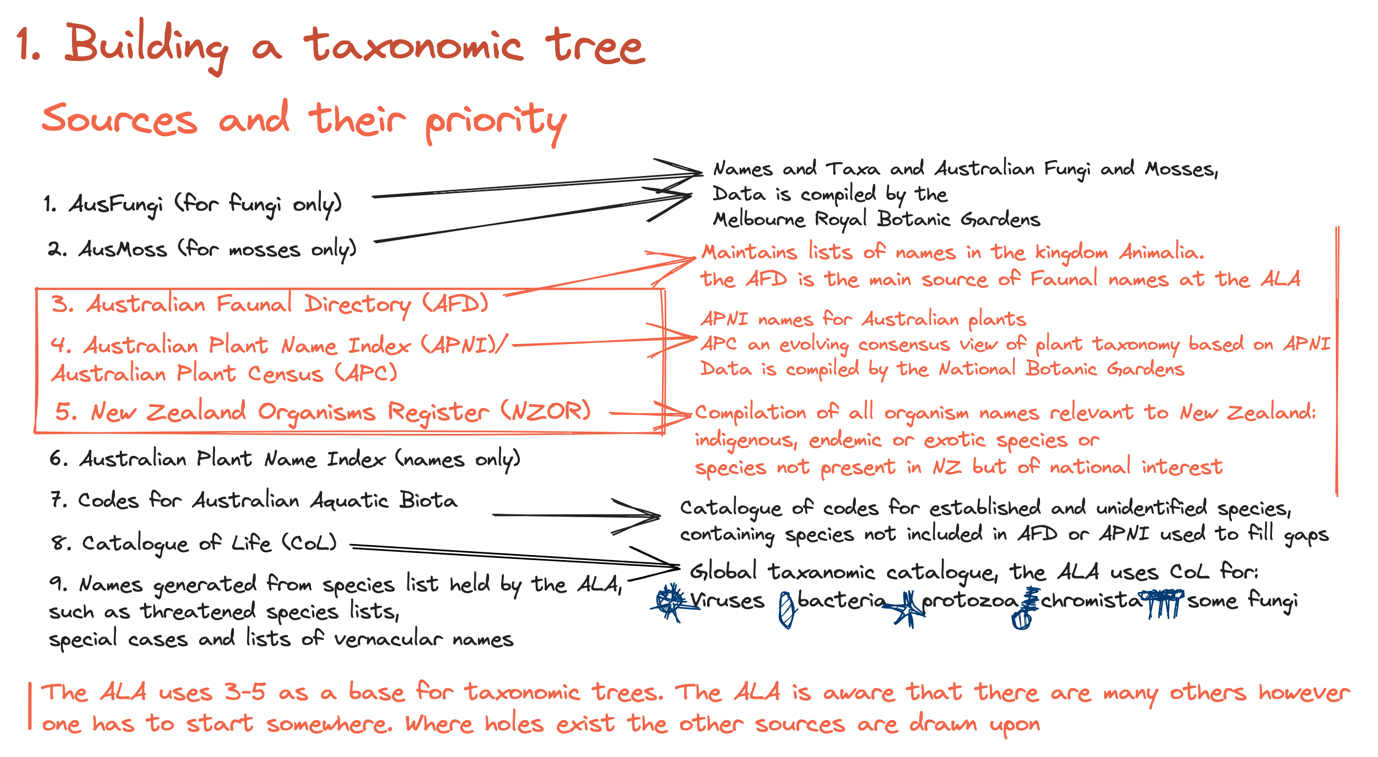
\includegraphics{./images/image-1066364510.png}

While this is in theory how the ALAs backbone is built, issues can occur
with aggregation leading to potentially serious problems with the
taxonomic structure. In addition data can be parsed incorrectly, and the
process isn't transparent. Meaning that when the taxonomic backbone is
updated, the elements that have changed are untraceable. These issues
are not specific to ALA taxonomy, but occur in varying forms among data
aggregators.

With all that, open source data has many pros, so how does one deal with
taxonomic inconsistencies to get the most accurate data in the end?

\hypertarget{choosing-your-own-naming-authority}{%
\subsection{Choosing your own naming
authority}\label{choosing-your-own-naming-authority}}

Using a naming authority is a great way to make decisions surrounding
taxonomic categorizations of open source biodiversity data. Accurate
species delimitation is crucial for adequate conservation management and
understanding evolutionary processes (Mace 2004). Species-level lists
are the foundation of conservation decisions, such as is the IUCN Red
List (\textbf{melville21?}). However, deciding what naming authority to
use can be challenging and time consuming.

What naming authority you choose can be dictated by:

\begin{enumerate}
\def\labelenumi{\arabic{enumi}.}
\tightlist
\item
  Are you looking at a single species, or single genus (Taxonomic)
\item
  Are you looking at all species in a certain region (spatial)
\end{enumerate}

The difference in scope might influence if you choose to use a naming
authority from a taxonomic society group or multiple broad sources.

A knowledge of taxonomy assist your ability to verify the data you are
working with. For this, different organizations provide updated lists of
species or even details of the taxonomic history of a species. Checking
changes in taxonomy can be helpful when interpreting old data which may
have species names you don't recognize. Changes in taxonomy, such as
species split, new higher level classification (as genera), or species
descriptions, highlight the importance of keeping up-to-date with
taxonomic literature. This can be achieved by consulting the literature.
Most taxonomic society groups release annual updates on taxonomy.

In Australia, the \href{https://www.anbg.gov.au/apni/}{Australian Plant
Name Index (APNI)} is the primary naming authority for plants. With the
\href{https://biodiversity.org.au/afd/home}{Australian Faunal Directory
(AFD)} the main taxonomic catalog for animal species. These authorities
provide a list of accepted and authoritative names as a template. If
you're unsure what naming authority to use and you're looking at
Australian species, the APNI and the AFD are a good place to start,
especially if the data you're investigating covers a wide range of taxa.
If you're investigating specific taxa it's worth checking when the
taxonomy was last updated in the APNI or AFD, especially if you know
there has been recent changes. If you want to investigate closer, we've
provided some links to society groups, in some cases these can be more
up to date that the APNI or AFD.

\hypertarget{australian-taxonomic-society-groups}{%
\subsection{Australian taxonomic society
groups}\label{australian-taxonomic-society-groups}}

\textbf{VERTEBRATES}

\begin{itemize}
\tightlist
\item
  Amphibians and reptiles - \href{https://ahs.org.au/}{Australian
  Herpetological Society}\\
\item
  Birds - \href{https://www.birdlife.org.au/}{Birdlife Australia}\\
\item
  Fish - \href{https://www.asfb.org.au/}{Australian Society for Fish
  Biology}\\
\item
  Mammals - \href{https://australianmammals.org.au/}{The Australian
  Mammal Society}
\end{itemize}

\textbf{INVERTEBRATES}

\begin{itemize}
\tightlist
\item
  Arachnology -
  \href{www.australasianarachnologicalsociety.org}{Australasian
  Arachnological Society}\\
\item
  Entomology - \href{https://www.austentsoc.org.au/}{Australian
  Entomological Society}\\
\item
  Malacology - \href{https://www.malsocaus.org/}{The Malacological
  Society of Australasia}\\
\item
  Nematology - \href{https://www.nematologists.org.au/}{Australasian
  Association of Nematologists}
\end{itemize}

\hypertarget{global-taxonomy}{%
\subsection{Global taxonomy}\label{global-taxonomy}}

\begin{itemize}
\item
  GBIF uses 100 different sources to assemble -
  \href{https://www.gbif.org/dataset/d7dddbf4-2cf0-4f39-9b2a-bb099caae36c}{their
  global taxonomic backbone}
\item
  Authoritative taxonomic information on plants, animals, fungi, and
  microbes - \href{https://www.itis.gov/}{Integrated Taxonomic
  Information System, ITIS}
\item
  Global taxonomic catalogue -
  \href{https://www.catalogueoflife.org/}{Catalogue of Life}
\end{itemize}

\hypertarget{what-to-do-with-the-naming-authority}{%
\section{What to do with the naming
authority}\label{what-to-do-with-the-naming-authority}}

Now that you've chosen a naming authority you can use it to ensure
consistency across your data set, but also check you haven't missed any
species data from your download.

\hypertarget{synonyms}{%
\section{Synonyms}\label{synonyms}}

There are two main types of taxonomic synonyms: \textbf{heterotypic} and
\textbf{homotypic.} The type of synonym might dictate how you handle it.

Homotypic: a name base on the same type as that of another name,
objective synonym {[}IAPT{]}

Heterotypic: a name based on a type different from that of another name
referring to the same taxon {[}IAPT{]}

Synonyms can be annoying to deal with when working with open source
data, and they can appear because of multiple reasons

\begin{enumerate}
\def\labelenumi{\arabic{enumi}.}
\tightlist
\item
  Taxonomy changes over time, a record from the 1950s might have a name
  that is no longer used for the species
\item
  The scientific community doesn't always agree, there may be multiple
  names, and taxonomic classifications for the same species
\end{enumerate}

Often naming authorities will have one they deem as accepted, and list
others as synonyms. Biodiversity data repositories will have a preferred
name according to the naming authority they use and display species data
under this name with synonyms listed. Sometimes data doesn't parse
correctly or maybe the data provider you're using recognizes the names
as different species. Because of this it can be worth with:

\begin{enumerate}
\def\labelenumi{\arabic{enumi}.}
\tightlist
\item
  Downloading higher taxon data and then filtering for what you need, as
  disparities are less common at higher levels
\item
  Include synonyms of the species names you're interested in your
  download
\item
  Download the original inputted name in fields such as
  ``verbatimScientificName'' which reflects a pre-parsed scientific
  name. This can be useful if conducting a spatial analyses
\end{enumerate}

Understanding if a species name has synonyms can also be useful for
accessing literature. For example some \emph{Eucaluptus} species have
been re-classified and old literature might refer to an old name you
were unaware of. This can increase your access to potentially seminal
literature about a species {[}REF{]}.

\hypertarget{standardize-taxonomy}{%
\section{Standardize taxonomy}\label{standardize-taxonomy}}

The following steps assume that the taxonomic history of the included
species is known and correct and out-of-date names and synonymy have
been fixed.

Ensure that the spelling is correct and fix errors as they appear. It is
essential to decide on a standard way to record the scientific names and
be consistent. For example, start with upper case and separate the names
with an underline e.g.~``Moloch\_horridus''.

It is also important to check the taxonomic hierarchy, make sure it's
correct and nothing is missing, such as family, and order. You can often
fill this information in using your chosen naming authority or referring
back to an atlas such as the ALA.

It's best practice to standardise and fix what you can before you start
removing anything, this decreases the chance of removing more records
than you need to.

\begin{itemize}
\item
  Remove non-identifiable specimens: If a species is not discernible
  after checking spelling and taxonomy, then it should be removed.
\item
  Remove records with insufficient taxon identification: If a record is
  not identified down to the species level and this level of detail is
  needed for the study, then the record should be removed.
\item
  Remove records with miss-identified taxonomy: Incorrectly identified
  species, or unrecognized species names compared to a naming authority,
  should be removed.

  Note: Incorrectly identified specimens can be difficult to identify
  with open source biodiversity data. Often these will be picked up by
  1) an image of the species in question which does not match 2) If you
  notice a species outside of its geographic range, this could be a true
  outlier, it could be a spatial error, or it could be a different
  species. (\textbf{see --- for more info})
\end{itemize}

\hypertarget{optional-taxonomic-cleaning}{%
\subsection{Optional taxonomic
cleaning}\label{optional-taxonomic-cleaning}}

The following steps may not apply to your research interests, however
this type of cleaning is commonly required.

\begin{itemize}
\item
  Remove non-native species: This step is a common requirement. A list
  can be obtained from the \href{https://griis.org/}{Global Register of
  Introduced and Invasive Species (GRIIS)}
\item
  Remove domesticated specimens, sightings of dogs, cats, but also
  garden species (\textbf{elaborate})
\item
  Remove extinct species: if you don't have a year filter on your data
  you might have records of species that have become extinct in more
  recent years.
\item
  Remove specific taxa/life stages depending on the study: For example,
  if working with terrestrial data, it is necessary to remove marine
  taxa.
\end{itemize}

\hypertarget{merge-datasets-from-different-infrastructures}{%
\section{Merge datasets from different
infrastructures}\label{merge-datasets-from-different-infrastructures}}

(Park this for now may come after naming authority)

If you have downloaded data from different sources, you likely will need
to collate your data into a singular database.

When combining data from multiple places, it is important to standardize
the data fields and merge the data carefully (Ribeiro et al. 2022).
There is a chance data will be incorrectly formatted and/or mislabeled.

One of the main issues you might face if you've sourced data from
different organisations/people is that higher taxonomy may not match- if
this is the case, take a look at the ``taxonomy'' chapter for more
information on how to deal with inconsistent taxonomy before merging!

\begin{Shaded}
\begin{Highlighting}[]
\DocumentationTok{\#\#example on formatting consistency, merging data together etc}
\end{Highlighting}
\end{Shaded}

\bookmarksetup{startatroot}

\hypertarget{sec-spatial}{%
\chapter{Spatial data}\label{sec-spatial}}

Now that you've been through the taxonomic cleaning steps it's time to
clean up the spatial element. Now is a great time to plot your data onto
a map again. Spatial errors are much easier to spot from a visual
perspective. You may have flagged some records as being taxonomically
incorrect, and it's important to keep those in mind as you go through
these steps, you might come across more.

\hypertarget{coordinate-correction}{%
\subsection{Coordinate correction}\label{coordinate-correction}}

(\textbf{some of this is in the download chapter-unsure if we want to
move it or keep it})

You may have already fixed up some of these when you first downloaded
your data, but now it's time to be more rigorous. As always we'll start
with fixing data before discarding, many coordinates issues can be
solved with data manipulation instead of discarding data:

\begin{itemize}
\item
  Correct flipped coordinates: Flipped coordinates typically appear as a
  clustering of points, whereby swapping the latitude and longitude will
  place the coordinates where they are expected.

  \emph{example map of some flipped coordinates (what to look for)}
\item
  Correct poorly formatted coordinates: Different datasets can provide
  coordinates in different formats, so it is crucial to correct the
  format of the coordinates before discarding any points.
\item
  Correct numerical sign confusion: As with flipped coordinates, if
  there is a clustering of points mirrored to another hemisphere,
  consider swapping the sign and correct rather than discarding the
  points.

  \emph{example map, like coordinates off the coast of japan}
\item
  Check for records with coordinates in a different country than is
  listed in the country field: The coordinates could be wrong or just
  the country listed. Note that the country should only be changed to
  match the coordinates if the data is trustworthy.
\item
  (\textbf{Correct/check for records with locality but no
  occurrence/georeference (if possible): If you have a good locality,
  consider georeferencing for coordinates rather than discarding the
  missing data entry. If the locality is not precise, this will likely
  yield lower-quality data points.}) unsure of this step if we want to
  go into georeferencing? or maybe point people to another resource
\end{itemize}

\hypertarget{coordinate-precision}{%
\subsection{Coordinate precision}\label{coordinate-precision}}

Open source biodiversity data will be collected from many people with
different tools and expertise, some record coordinates may have been
recorded with a phone, some with a GPS, and some maybe just from a place
name and coordinates added after the fact. Depending on the level of
precision you need, you might consider discarding data that is not
precise enough, or removing decimal places for data you know could not
be that precise. At the ALA there is a ``cooridnateprecision''/
``coordinateUncertainityIn Meters'' column you can download with the
data which can sometime help discern the accuracy of the data (worth
noting it's not always completed).

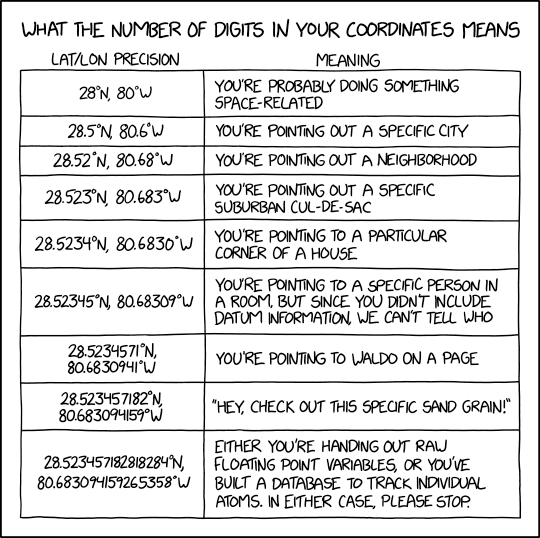
\includegraphics{./images/image-613988507.png}

https://xkcd.wtf/2170/

Realistically you will probably be working with between 2 and 5 decimal
places. Studies often have different precision cut-offs. For example,
coordinate precision below 100km represents the grain size of many
macroecological analyses. Some studies have used a cut-off of spatial
resolution \textgreater25,000m or precision with less than three decimal
places (\textbf{add a reference here}). It is important to note that
rasterized collections often have a significant proportion of records
that might have low coordinate precision. Understanding the level of
quality you need is important before removing/keeping large volumes of
data.

\begin{itemize}
\item
  How to filter by \# of decimal places
\end{itemize}

\hypertarget{coordinate-cleaning}{%
\subsection{Coordinate cleaning}\label{coordinate-cleaning}}

Now that you've gone through and fixed what you can, it's time to remove
records that still have errors. This doesn't mean removing outliers,
we'll talk about those later.

\begin{itemize}
\item
  Remove records with null or missing coordinates. This will be records
  missing partial or complete information. Missing values can cause
  errors, many analytical tools do not respond well to missing values.
  If you can't find the information elsewhere, it's best to remove it.
\item
  Remove records where longitude and latitude are equal: High likelihood
  that this is not where the record was recorded and, therefore, should
  be checked and (possibly) removed.
\item
  Remove records with zero coordinates {[}that could not be
  georeferenced{]}: When plotting it on a map, zero coordinates will be
  found around the point at zero latitudes and longitudes. These records
  will not accurately represent their valid location and must be
  removed.
\item
  Remove records plotted away from the known area of distribution of the
  species. It is essential to check the metadata to ensure that it is a
  data entry error and not a real outlier. In some cases, it's worth
  checking the literature before discarding records like these. These
  can also be mis-identified species, if you're working with data from
  many species, and you find a species point in amongst the
  environmental bounds of a similar looking species it might be worth
  going back to the original record and taking a closer look. However,
  if no images exist it might be difficult to determine if it is a
  taxonomic or spatial issue.

  There are several ways of dealing with this issue, but one option can
  be to mask data to remove points from falling off a determined area.
\item
  Remove records with coordinates assigned to country and province
  centroids: There are many fonts that deal with centroid data, such as
  Centre of Country, botanic gardens, zoos, country capitals,
  biodiversity institutions, urban areas, and gbif headquarters. This
  issue can happen for several reasons and sometimes can be tricky to
  spot. Exploratory visuals can help support findings, making it easier
  to spot clusterings of points.

  Centroids are common when records are being assigned from
  georeferencing based on vague locality descriptions or from incorrect
  georeferencing. Sometimes, records are erroneously entered with the
  physical location of the specimen or because they represent
  individuals from captivity or horticulture, which were not clearly
  labeled as such.

  In a few cases, zoos and botanic gardens might be where the record was
  sighted. However, in this case, it is not naturally occurring and
  should be removed. Records in urban areas may not want to be removed
  by everyone, but it is essential to note that it could be old data or
  have vague locality descriptions.
\end{itemize}

\begin{itemize}
\tightlist
\item
  Remove records outside of the country of interest: In some cases,
  records outside the country of origin may be outliers. In other cases,
  they may be perfectly valid. It is important to analyze case-by-case
  and remove the record if necessary.
\end{itemize}

\hypertarget{checklist-of-data-standardization}{%
\section{Checklist of data
standardization}\label{checklist-of-data-standardization}}

Add here a downloadable checklist of issues to be checked.

\bookmarksetup{startatroot}

\hypertarget{duplicates}{%
\chapter{Duplicates}\label{duplicates}}

Duplicates add computational burden to your analyses. Some spatial
analyses won't run if duplicates are present as it breaks mathematical
constraints. There are a few different categories of duplicates which
you might encounter when working with open source biodiversity data,
with some being more difficult to work with than others.

\begin{enumerate}
\def\labelenumi{\arabic{enumi}.}
\item
  True duplicates = Unique identifier (UID) is the same

  True duplicates can occur for many reasons, often data is sent to the
  state authority it was collected in as well as the authority
  responsible for collecting the data, which is not always the same.
  When this data is aggregated by the ALA for example, they end up with
  multiple copies. These are true duplicates- as in they have the same
  UID, same coordinates, same species. They don't always impact
  modelling. Although they can impact sampling bias and increase
  computational burden for no added benefit so it's best to remove them
  (Jin and Yang 2020; J. R. Marsh et al. 2022).

  Removing true duplicates where the UID is the same is quite
  straightforward and is a common step before mapping biodiversity data.
\item
  Different UID Same species, same coordinates, yet different year.

  If the UID is different, but the species name is the same and the
  coordinates are the same this could be a couple of different things:

  a) If the year is different, it's likely a true record, indicating
  it's continued presence- this is most likely for plants\ldots there
  are cases where you'll still want to remove the

  b) Herbarium duplicates: same year, same collector, however different
  UID and minor differences in locality, coordinate precision. These can
  be more difficult to decipher, and we've called them Herbarium
  duplicates as this is when they most commonly occur. The same specimen
  will sometimes be sent to multiple herbariums, this results in
  different UIDs. Additionally because the data is potentially being
  inputted by different people the discrepancies this causes can make
  them difficult to spot {[}REF bob pers com{]}.

  \#\#example from bobs data
\item
  Spatial thinning = records located close to each other

  These records are not duplicates, not the same individual, not in
  exactly the same spot, yet close together. Think about patch of grass,
  this isn't one plant but many all packed tightly together. This adds
  computational burden, especially for large scale biodiversity analyses
  and distribution modelling for many species (Zizka et al. 2020b;
  Kuralt, n.d.). This can also be done to reduce bias associated with
  oversampling at a small number of sites within larger species ranges
  (Godfree et al. 2021).
\end{enumerate}

\bookmarksetup{startatroot}

\hypertarget{outliers-and-final-checks}{%
\chapter{Outliers and final checks}\label{outliers-and-final-checks}}

\#note from meeting with Martin this section might include some alpha
hull examples for how to detect outliers, or how they can skew your
data, in addition to maybe an SDM for outlier detection (Simões and
Peterson 2018) even if we won't be teaching people how to run an SDM

Outliers can be true outliers or data errors, true outliers are not
necessarily to be removed. This could represent mis-identified
specimens, etc

(\#note to double check what i wrote for support article around
inconsistent sampling and open source data)

\bookmarksetup{startatroot}

\hypertarget{work-example}{%
\chapter{Work Example}\label{work-example}}

Include here an workable example (maybe using galah?)

\bookmarksetup{startatroot}

\hypertarget{summary}{%
\chapter{Summary}\label{summary}}

\begin{itemize}
\tightlist
\item
  nice diagram
\item
  decide where to refer to the R packages
\item
  add references
\end{itemize}

\hypertarget{extra-notes}{%
\section{Extra notes}\label{extra-notes}}

Now that the data is cleaned and standardized, extra work can be done to
guarantee the data quality. These steps will depend on the kind of study
being conducted.

\begin{itemize}
\item
  Remove duplicates: Data duplication is common when combining data from
  multiple sources. In most part of the cases, you will want to remove
  duplicate data, as it just increase you data size without bringing in
  any relevant information. It can also make analysis faster and more
  efficient.
\item
  Bias correction: Account for sampling bias.
\item
  Scrutinise outliers: Outliers can be true outliers or data errors.
  True outliers are not necessarily to be removed. This could represent
  misidentified specimens, etc.
\item
  Format data: Subset, specify data source as ALA, indicate sensitive
  species, assign habitat column, rearrange and name columns.
\item
  Study region: Important if you need to crop data to the region or to
  work out the current range, background region, and projection region.
\item
  Assign quality levels to data: If you need help with specific data,
  assigning quality level metrics for taxonomy and geographical
  dimensions can be good.
\item
  Manually identify and remove false positives: False positives that may
  have been overlooked by automated error removal, based on the
  knowledge that they are in the records.
\item
  Remove records with an individual count of less than 1 or more than
  99: Records may be unsuitable if the number of recorded individuals is
  0 or the count is too high (data entry or data-basing problems),
  indicate records from dna barcoding and in some cases indicate records
  of absence.
\item
  Consider species with fewer records: Depending of the the type of
  analysis to be conducted, as in the case of Species Distribution
  Modelling, the number of distribution points available can influence
  the quality of the results.
\item
  Reach out and ask questions: When preparing occurrence data for
  modeling it can be helpful to speak to experts in the field.
\end{itemize}

\bookmarksetup{startatroot}

\hypertarget{sec-appendix}{%
\chapter{Appendix}\label{sec-appendix}}

We don't claim to be experts in data cleaning, therefore in order to
ensure content for this book was current and relevant we undertook an
informal literature review of both peer reviewed and grey literature.
Key themes searched were:

\begin{enumerate}
\def\labelenumi{\arabic{enumi}.}
\item
  Cleaning data for species distribution models
\item
  Cleaning open biodiversity data
\item
  Australian and global naming authorities
\item
  R packages for biodiversity data cleaning
\end{enumerate}

As this was not a comprehensive literature review recent papers were
selected first as the R environment is a rapidly evolving space. Methods
sections outlining data cleaning protocols were read and collated into a
database. Papers which were frequently referenced were also chosen for
review in order to not miss older seminal papers. Additionally our
project partners outputs (J. Marsh et al. 2021; Godfree et al. 2021)
have been investigated in detail to understand and streamline their data
cleaning processes. This has included detailed review of their code base
as well as meetings with the authors of the papers to understand their
processes, issues and needs.

All steps for acquiring and cleaning data were then looked at together
in order to understand what were essential steps, versus what was done
in certain use cases. We also investigated the order in which steps were
undertaken to develop the most streamlined process for this book.

\bookmarksetup{startatroot}

\hypertarget{sec-references}{%
\chapter{References}\label{sec-references}}

\hypertarget{refs}{}
\begin{CSLReferences}{1}{0}
\leavevmode\vadjust pre{\hypertarget{ref-fuhrding-potschkat_influence_2022}{}}%
Führding-Potschkat, Petra, Holger Kreft, and Stefanie M. Ickert-Bond.
2022. {``Influence of Different Data Cleaning Solutions of
Point-Occurrence Records on Downstream Macroecological Diversity
Models.''} \emph{Ecology and Evolution} 12 (8): e9168.
\url{https://doi.org/10.1002/ece3.9168}.

\leavevmode\vadjust pre{\hypertarget{ref-garraffoni2019integrative}{}}%
Garraffoni, André RS, Thiago Q Araújo, Anete P Lourenço, Loretta Guidi,
and Maria Balsamo. 2019. {``Integrative Taxonomy of a New Redudasys
Species (Gastrotricha: Macrodasyida) Sheds Light on the Invasion of
Fresh Water Habitats by Macrodasyids.''} \emph{Scientific Reports} 9
(1): 2067.

\leavevmode\vadjust pre{\hypertarget{ref-godfree_implications_2021}{}}%
Godfree, Robert C., Nunzio Knerr, Francisco Encinas-Viso, David
Albrecht, David Bush, D. Christine Cargill, Mark Clements, et al. 2021.
{``Implications of the 2019--2020 Megafires for the Biogeography and
Conservation of {Australian} Vegetation.''} \emph{Nature Communications}
12 (1): 1023. \url{https://doi.org/10.1038/s41467-021-21266-5}.

\leavevmode\vadjust pre{\hypertarget{ref-gueta_quantifying_2016}{}}%
Gueta, Tomer, and Yohay Carmel. 2016. {``Quantifying the Value of
User-Level Data Cleaning for Big Data: {A} Case Study Using Mammal
Distribution Models.''} \emph{Ecological Informatics} 34 (July):
139--45. \url{https://doi.org/10.1016/j.ecoinf.2016.06.001}.

\leavevmode\vadjust pre{\hypertarget{ref-jin_bdcleaner_2020}{}}%
Jin, Jing, and Jun Yang. 2020. {``{BDcleaner}: {A} Workflow for Cleaning
Taxonomic and Geographic Errors in Occurrence Data Archived in
Biodiversity Databases.''} \emph{Global Ecology and Conservation} 21
(March): e00852. \url{https://doi.org/10.1016/j.gecco.2019.e00852}.

\leavevmode\vadjust pre{\hypertarget{ref-kuralt}{}}%
Kuralt, Zan. n.d. {``GBIF Data for Species Distribution Modelling: A
Case Study of Lithobius Erythrocephalus (Chilopoda: Lithobiidae).''}
\url{http://rstudio-pubs-static.s3.amazonaws.com/415459_61fae98ff3984241bd5f7f31da425c98.html}.

\leavevmode\vadjust pre{\hypertarget{ref-mace2004role}{}}%
Mace, Georgina M. 2004. {``The Role of Taxonomy in Species
Conservation.''} \emph{Philosophical Transactions of the Royal Society
of London. Series B: Biological Sciences} 359 (1444): 711--19.

\leavevmode\vadjust pre{\hypertarget{ref-marsh2021}{}}%
Marsh, Jess, Payal Bal, Hannah Fraser, Kate Umbers, Aaron Greenville,
Libby Rumpff, and John Woinarski. 2021. {``Assessment of the Impacts of
the 2019-20 Wildfires of Southern and Eastern Australia on Invertebrate
Species Final Report.''}

\leavevmode\vadjust pre{\hypertarget{ref-marsh_accounting_2022}{}}%
Marsh, Jessica R., Payal Bal, Hannah Fraser, Kate Umbers, Tanya Latty,
Aaron Greenville, Libby Rumpff, and John C. Z. Woinarski. 2022.
{``Accounting for the Neglected: {Invertebrate} Species and the
2019--2020 {Australian} Megafires.''} \emph{Global Ecology and
Biogeography} n/a (n/a). \url{https://doi.org/10.1111/geb.13550}.

\leavevmode\vadjust pre{\hypertarget{ref-ribeiro_bdc_2022}{}}%
Ribeiro, Bruno R., Santiago José Elías Velazco, Karlo Guidoni-Martins,
Geiziane Tessarolo, Lucas Jardim, Steven P. Bachman, and Rafael Loyola.
2022. {``Bdc: {A} Toolkit for Standardizing, Integrating and Cleaning
Biodiversity Data.''} \emph{Methods in Ecology and Evolution} 13 (7):
1421--28. \url{https://doi.org/10.1111/2041-210X.13868}.

\leavevmode\vadjust pre{\hypertarget{ref-rodrigues_species_2022}{}}%
Rodrigues, Arthur Vinicius, Gabriel Nakamura, Vanessa Graziele
Staggemeier, and Leandro Duarte. 2022. {``Species Misidentification
Affects Biodiversity Metrics: {Dealing} with This Issue Using the New
{R} Package {naturaList}.''} \emph{Ecological Informatics} 69 (July):
101625. \url{https://doi.org/10.1016/j.ecoinf.2022.101625}.

\leavevmode\vadjust pre{\hypertarget{ref-simoes2018utility}{}}%
Simões, Marianna VP, and A Townsend Peterson. 2018. {``Utility and
Limitations of Climate-Matching Approaches in Detecting Different Types
of Spatial Errors in Biodiversity Data.''} \emph{Insect Conservation and
Diversity} 11 (5): 407--14.

\leavevmode\vadjust pre{\hypertarget{ref-streamdna_sharing_2020}{}}%
streamdna. 2020. {``Sharing Is {Caring}: {Working} with {Other} People's
{Data}.''}
\url{https://methodsblog.com/2020/09/04/sharing-is-caring-working-with-other-peoples-data/}.

\leavevmode\vadjust pre{\hypertarget{ref-zizka_no_2020}{}}%
Zizka, Alexander, Fernanda Antunes Carvalho, Alice Calvente, Mabel Rocio
Baez-Lizarazo, Andressa Cabral, Jéssica Fernanda Ramos Coelho, Matheus
Colli-Silva, Mariana Ramos Fantinati, Moabe F Fernandes, and Thais
Ferreira-Araújo. 2020a. {``No One-Size-Fits-All Solution to Clean
{GBIF}.''} \emph{PeerJ} 8: e9916.

\leavevmode\vadjust pre{\hypertarget{ref-zizka2020}{}}%
---------. 2020b. {``No One-Size-Fits-All Solution to Clean GBIF.''}
\emph{PeerJ} 8: e9916.

\end{CSLReferences}



\end{document}
